\chapter{Analysis}
\label{chapter:ldmx:analysis}

One of the primary strengths of the \ac{ldmx} detector design is its ability to use the tagging and
recoil tracker system to reject a large number of background events by separating a nominal beam
with non-standard energy loss from a nominal beam with standard energy loss or even low-energy
beam. Moreover, the tagging and recoil tracker system gives \ac{ldmx} the potential to further
suppress backgrounds or potentially study \ac{dm} properties by studying the transverse momenta of
electrons recoiling from dark-bremsstrahlung candidate events.

While this design is optimal for a large number of \ac{eot}, the strategy has some limitations for
a low \ac{eot} data run. To limit multiple scattering which ruins momentum measurements, the
baseline detector configuration requires a thin ($\approx 0.1\mathrm{X}_0$) target. In the early
stages of \ac{ldmx}, when the total \ac{eot} will be lower, a different analysis strategy and
detector configuration may be optimal to probe the largest amount of the $y$--$m_\chi$ phase
space.\todo[introduce]{Provide MM search reach to help give conext to y and mchi.} The alternative
strategy ignores the dedicated target inside the tracker volume and instead uses the \ac{ecal}
as an active target. The \ac{eat} analysis channel for \ac{ldmx} thus has two primary purposes
which can be separated by the timeline over which they are relevant.
\begin{enumerate}
  \item \textbf{Short Term}: In early running, when the number of \ac{eot} is
        relatively small, the nominal \ac{mm} analysis will not have obtained
        significant reach into new \ac{dm} phase space (yet). The \ac{eat} channel
        serves here as a way to obtain world-leading sensitivity early in the lifetime
        of \ac{ldmx} and give the collaboration a first look at the data the apparatus
        has collected.
  \item \textbf{Long Term}: As \ac{ldmx} collects data, the \ac{mm}
        analysis enters into unexplored phase space and serves as a better discovery
        mechanism due to its access to the Tagger and Recoil trackers. The \ac{eat}
        channel, while struggling to suppress complicated backgrounds with relatively
        limited analysis handles, can operate ``orthogonally'' in the collected data
        since its primary selection (an approximately beam-energy electron passing
        through the Recoil tracker) is inverted relative to the \ac{mm} analysis
        (the electron passing through the Recoil tracker has significantly less
        energy than the beam).
\end{enumerate}

An initial study of the \ac{eat} analysis channel is the primary focus of \cref{part:ldmx} of this
thesis, focusing primarily on the first (short term) purpose. In this regard, we target an \ac{eot}
that is reasonable to accomplish early in the running of \ac{ldmx} and avoids particularly
intricate backgrounds. A total of \num{1e13} \ac{eot} fits these requirements by avoiding the
charged current production of neutrinos and represents $\sim\qty{10}{\percent}$
of the first full \ac{ldmx} dataset which is obtainable within approximately a two weeks
of nominal beam time\footnote{%
  Assuming the \ac{ldmx} detector apparatus and beam delivery is operating according to specifications,
  we expect the beam to be delivered on a frequency of \qty{37.5}{\mega\hertz} with a duty cycle of $\approx$\num{0.5} and the
  number of electrons within each bunch to be Poisson distributed with $\mu=1$.
  $\qty{37.5}{\mega\hertz}\times0.5\times P(\mu=1,1) \times\qty{2}{week}\approx\num{1e13}$~\ac{eot}.
}. Since \ac{eat} is expected to be the \emph{first} physics analysis on \ac{ldmx} data, we want a
\emph{simple} and \emph{robust} analysis that can withstand the test of time and the complexities
of real data.

With these design goals in mind, a simple ``cut-and-count'' analysis has been developed. The
simplicity of this analysis is one of its strengths, enabling it to be applicable despite potential
surprises arising from first encounters with real data. The bulk of time and effort on this first
investigation was focused on making this investigation \emph{possible} via the introduction of
midshower process filtering and a dark bremsstrahlung simulatin process described in
\cref{chapter:ldmx:simulation}.

\section{Selection}
The core goal of most search analyses is to develop a selection that avoids events known to be
standard processes (i.e. backgrounds) while keeping events containing the process being searched
for (in this case, the production of \ac{dm} via dark-bremsstrahlung).
Both the \ac{eat} analysis channel and the primary \ac{mm} channel share the dark-bremsstrahlung
signature of missing energy within the \ac{ecal} relative to the known incident beam energy.
This allows for the first selection made to be shared between these two channels -- 
a requirement that the sum of the observed energy in the first twenty layers of the \ac{ecal}
is less than \qty{1.5}{\GeV} (\qty{3.16}{\GeV}) for a \qty{4}{\GeV} (\qty{8}{\GeV}) beam.
This preliminary selection acts as the primary trigger for both of these analyses --
selecting events that resemble dark-bremsstrahlung via their lower-than-average
observed energy during data collection -- however, the \ac{eat} analysis channel in the early-running
scenario may not be collecting data with a fully calibrated energy scale at the trigger level.
The potential for mis-calibration motivates tightening the analysis missing energy requirement
by \qty{400}{\mega\electronvolt} as well as requiring the sum to be performed over all thirty-four
layers of the \ac{ecal} instead of only the first twenty.
\cref{fig:energy-after-trigger} shows the unit-normalized distributions of this total reconstructed
energy within the \ac{ecal} after the trigger has been applied.

\begin{figure}[htb]
    \centering
    \begin{subfigure}{0.48\textwidth}
         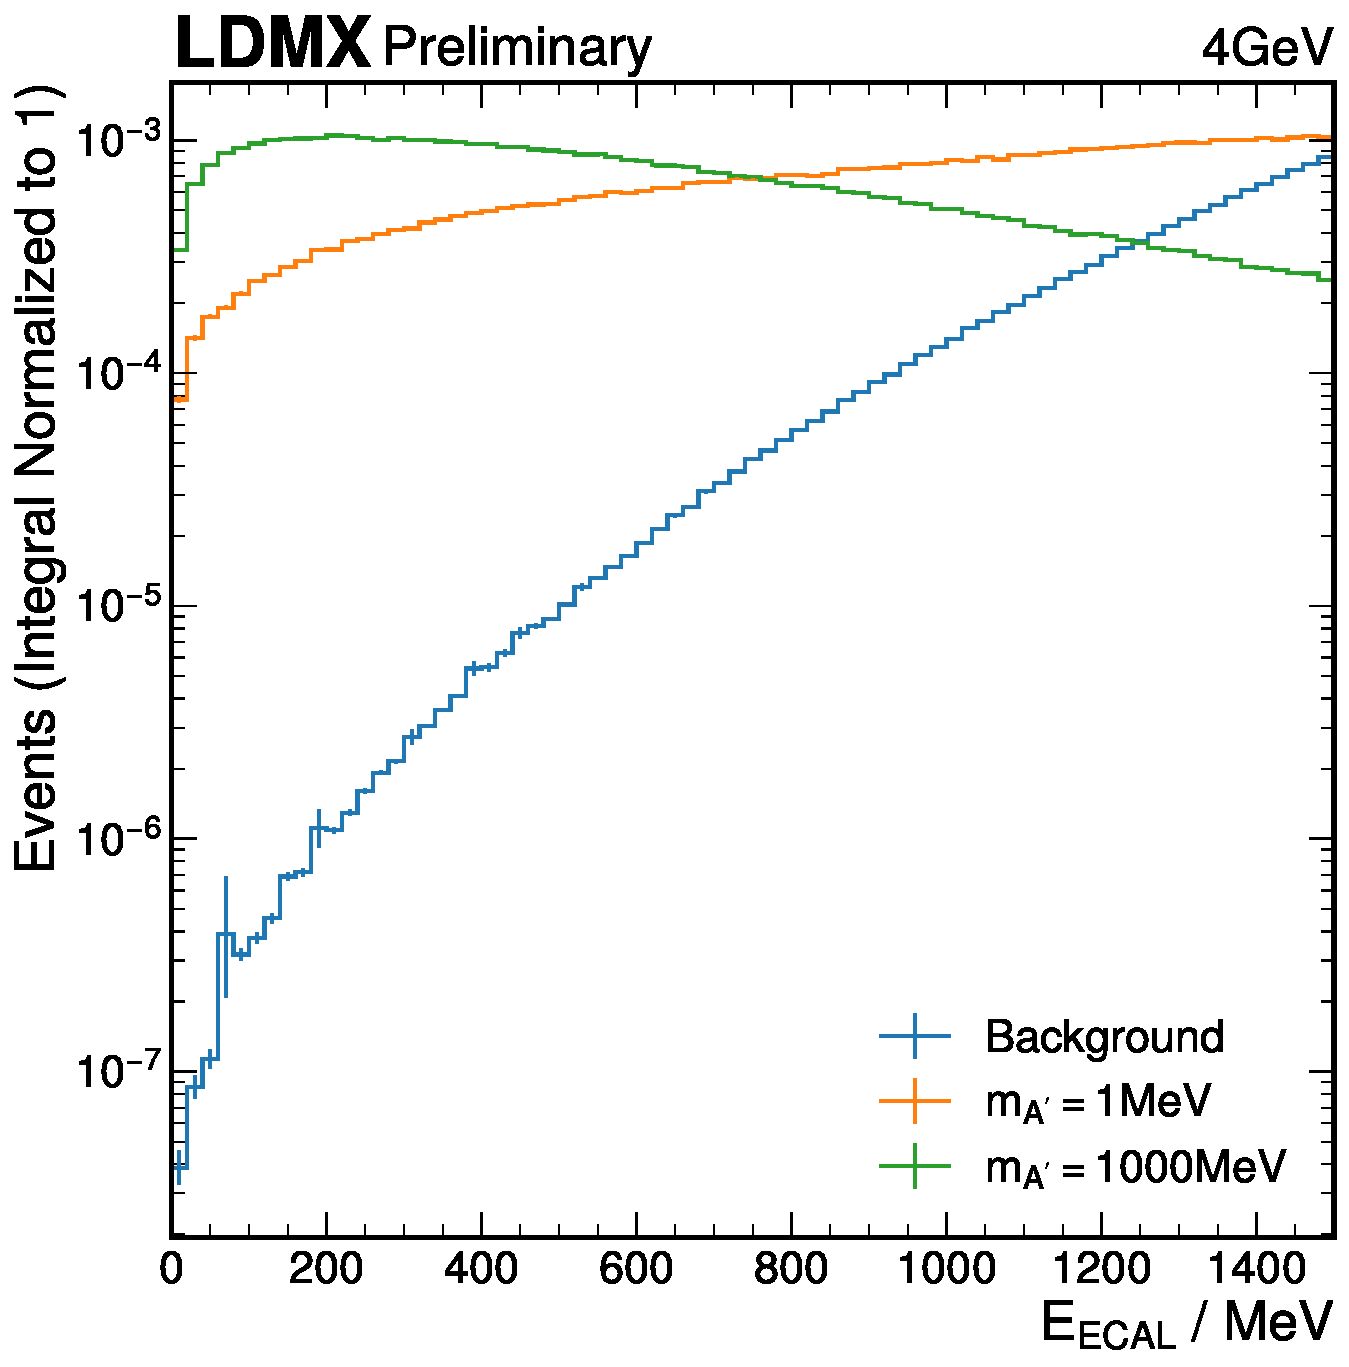
\includegraphics[width=\textwidth]{%
           figures/ldmx/analysis/energy-after-trigger-4gev.pdf}
    \end{subfigure}
    ~
    \begin{subfigure}{0.48\textwidth}
         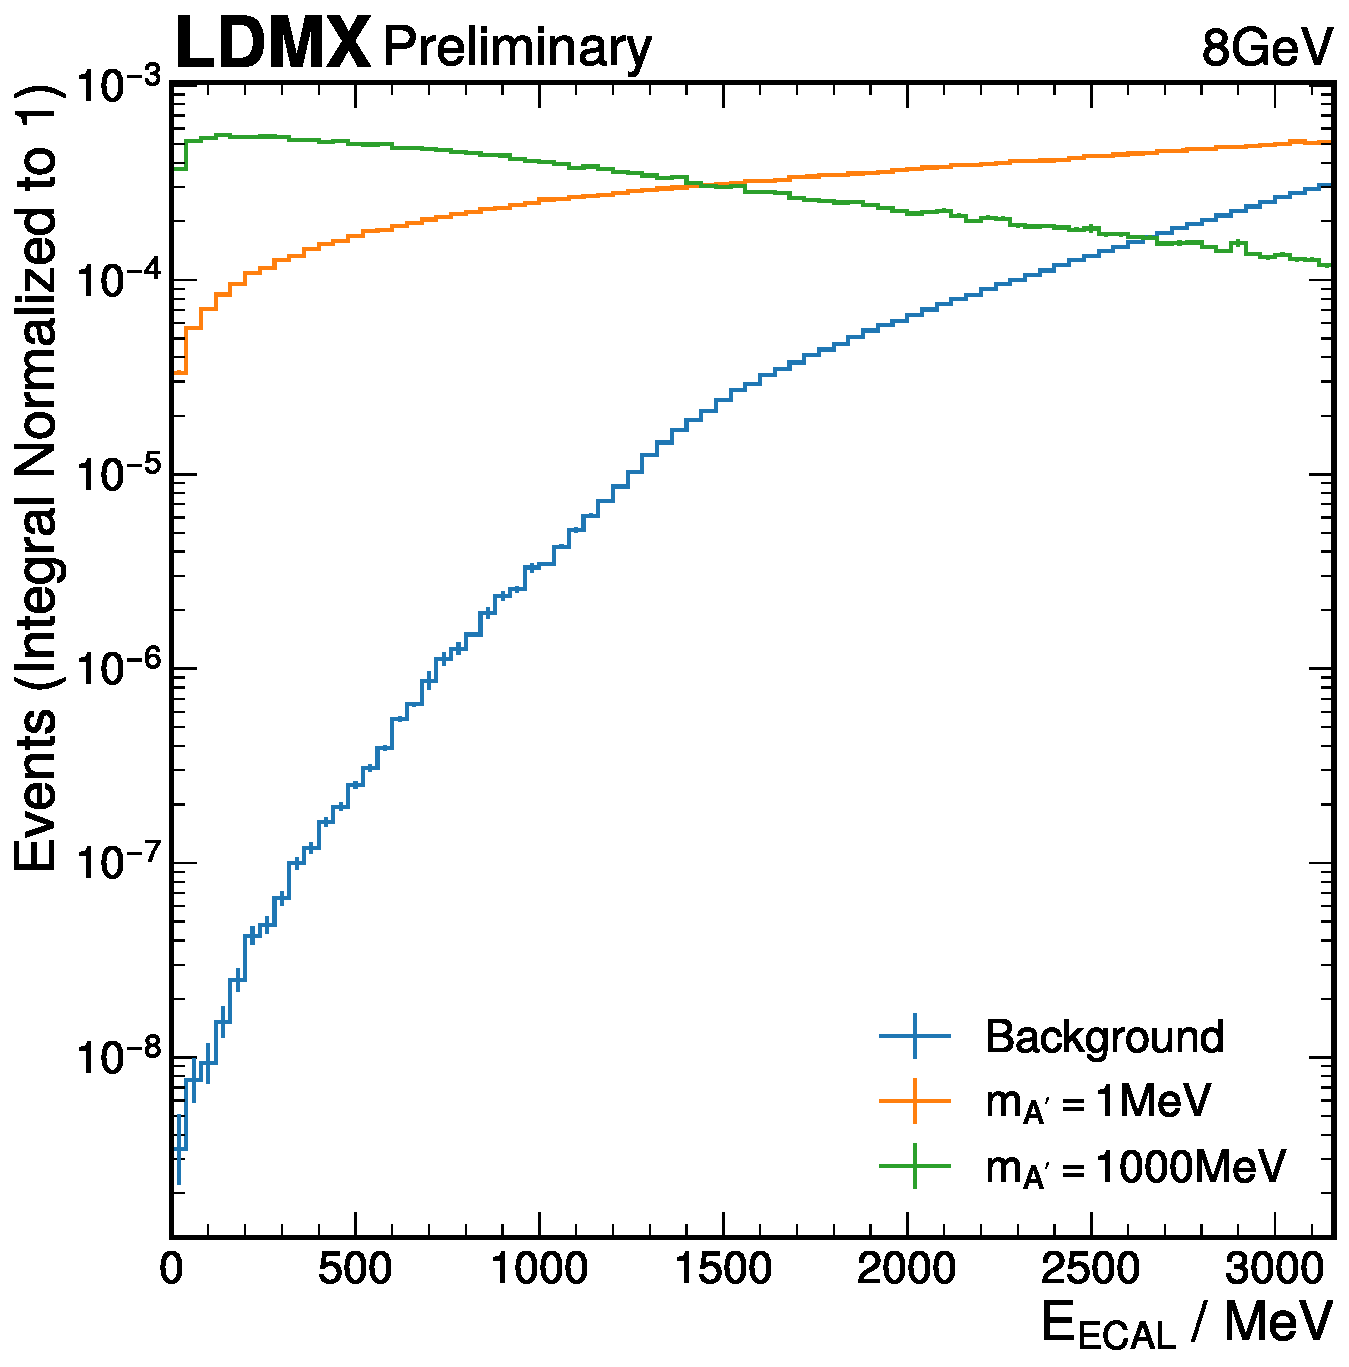
\includegraphics[width=\textwidth]{%
           figures/ldmx/analysis/energy-after-trigger-8gev.pdf}
    \end{subfigure}
    \caption{
    The total reconstructed energy in all layers of the ECal ($E_\text{ECAL}$).
    The signal and background distributions are normalized such that their integral is one.
    The \qty{4}{\GeV} beam is shown on the left and the \qty{8}{\GeV} beam is shown
    on the right.
    The events falling into bins with $E_\text{ECAL} > \qty{1.5}{\GeV}~(\qty{3.16}{\GeV})$
    for \qty{4}{\GeV} (\qty{8}{GeV}) are omitted from this plot but included in efficiency calculations.
    }
    \label{fig:energy-after-trigger}
\end{figure}

After this total energy requirement, there are still backgrounds left and those that remain are largely
events where a significant fraction of the energy is carried by particles difficult to contain (or even observe)
within the \ac{ecal} (neutrons, $K_L$, or muons for example).
To suppress these types of persistent backgrounds, the event is required to have less than 10 photoelectrons
deposited in any single bar of the \ac{hcal} -- $\max(\mathrm{PE}_\mathrm{HCal}) < 10$ --
well below the typical signal of a through-going muon of 80 photoelectrons in any single bar.

While this selection does a good job of removing events containing long-living particles, there are some
events containing several low-energy particles that range out within the \ac{ecal} itself.
These particles (often due to their number) distribute energy over a range of cells,
so we can suppress these events by requiring the spatial distribution of energy within the \ac{ecal} to be small.
We choose to measure the spatial distribution using the energy-weighted root-mean-squared spread of the
hits within the \ac{ecal}\footnote{
  A ``hit'' is defined as a single cell within the \ac{ecal} registering a signal corresponding to 50\% (or more)
  of the energy deposited by a typical muon during the event.
}
-- the \ac{ecal} Hit RMS -- which is typically larger for these background processes than for a single,
truncated electromagnetic shower present within a signal event.
We therefore require the \ac{ecal} Hit RMS to be less than \qty{20}{\mm}.

These two selection variables are shown in \cref{fig:selection-variables}
where the distributions are shown after all other selections are applied
(including the trigger selection and the tighter selection on the total \ac{ecal} energy including all layers).
\cref{tab:cutflow} shows the tabulation of this selection for the studied simulation samples.
\cref{fig:final-selection} shows the signal and background total \ac{ecal} energy distributions after
these selections are applied where we can still observe difference in the shapes of these distributions which
we will exploit in the final statistical analysis of these samples.

\begin{figure}
    \centering
    \begin{subfigure}{0.48\textwidth}
      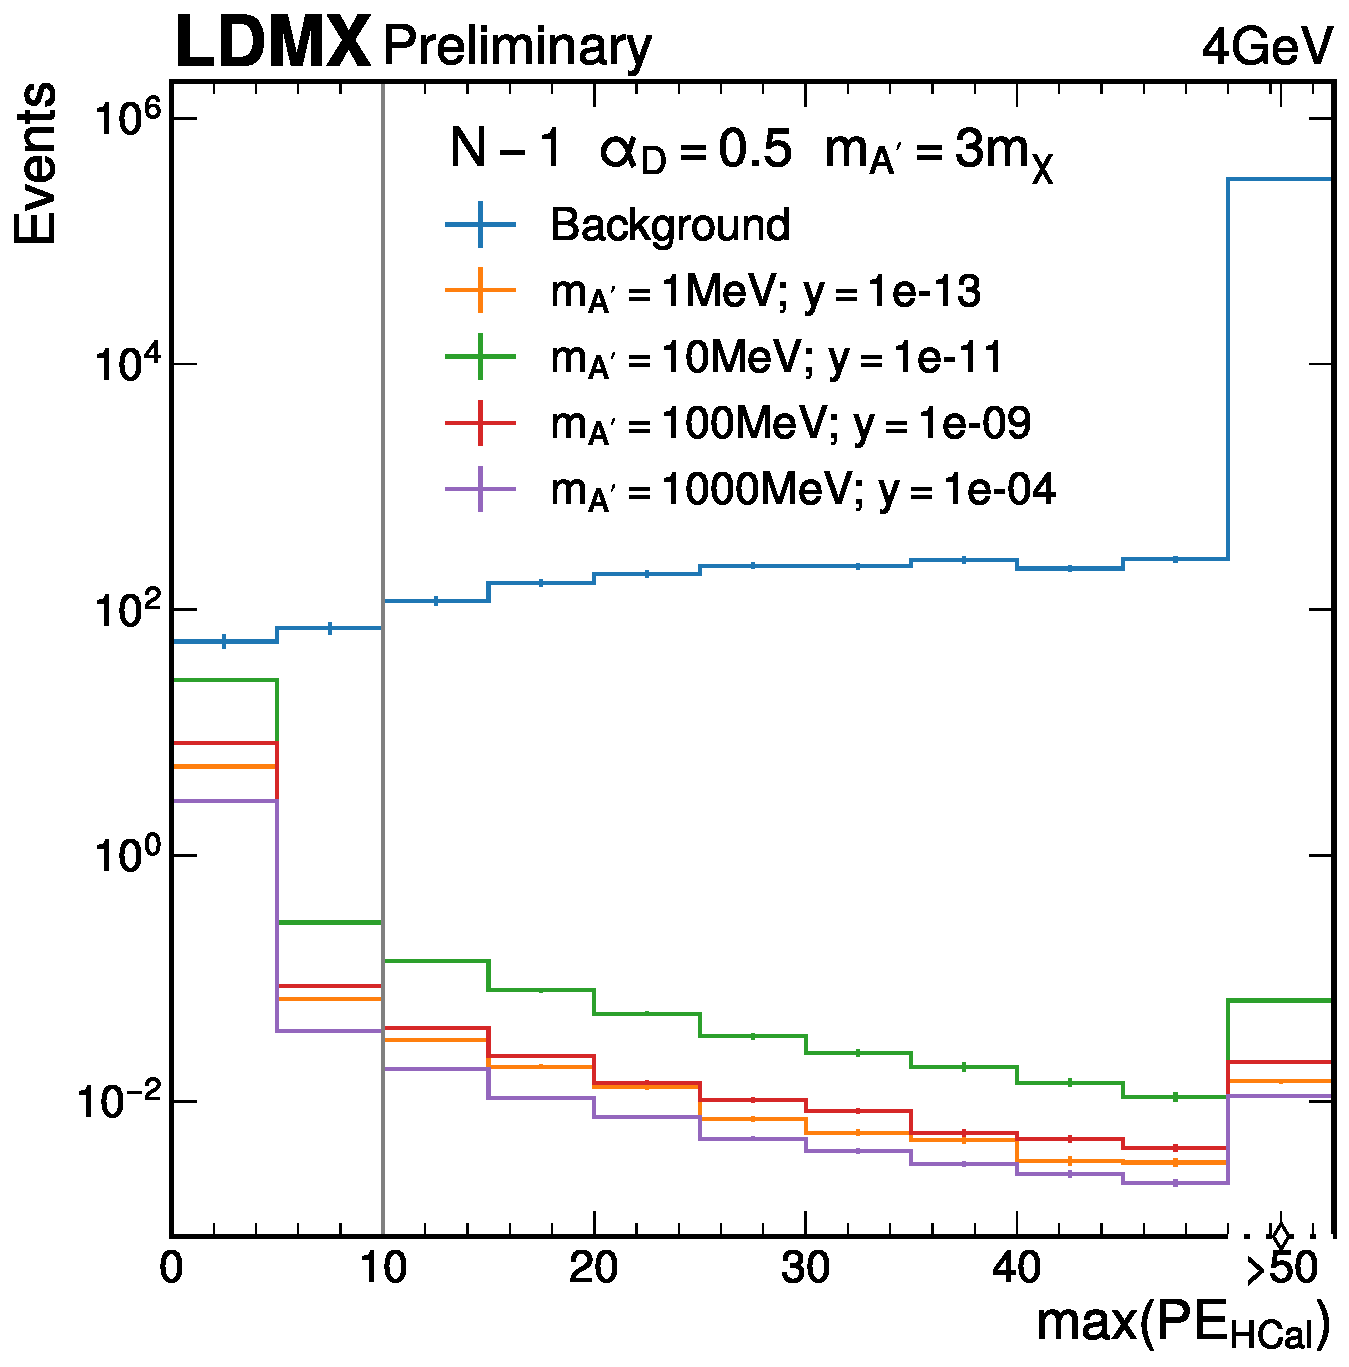
\includegraphics[width=\textwidth]{figures/ldmx/analysis/nm1-hcal-max-pe-4gev-1e13norm.pdf}
    \end{subfigure}
    ~
    \begin{subfigure}{0.48\textwidth}
      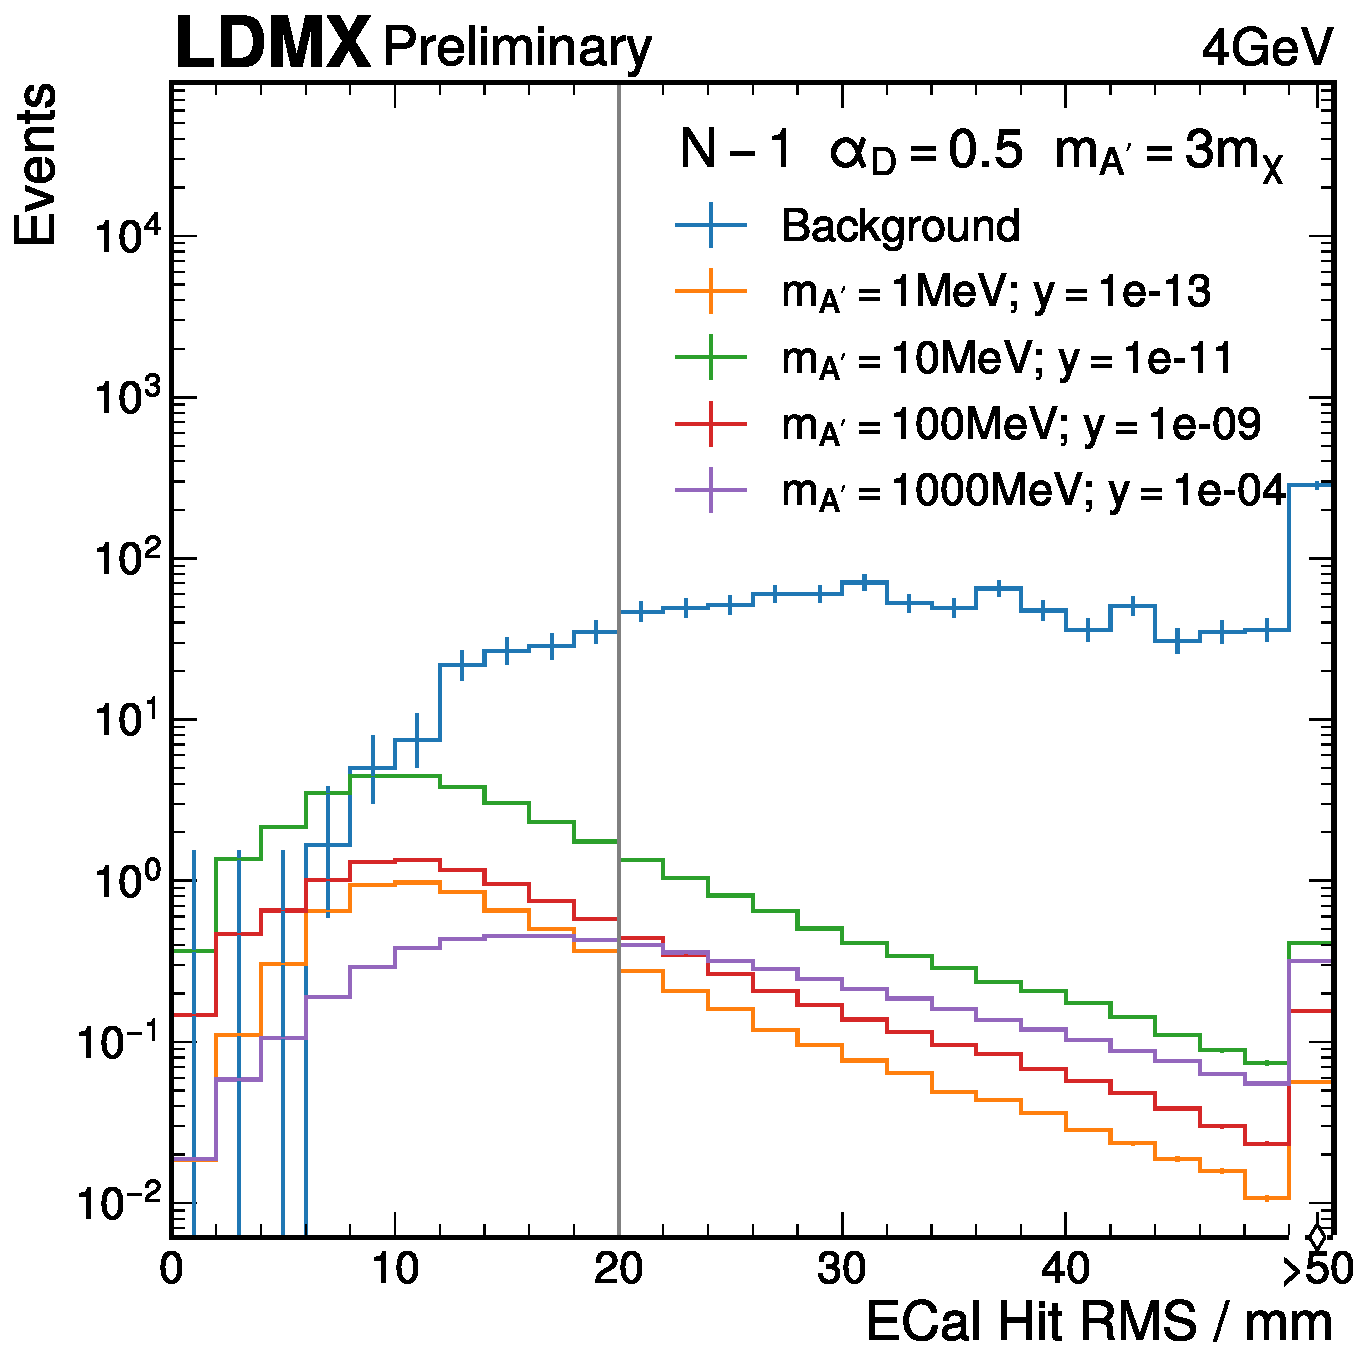
\includegraphics[width=\textwidth]{figures/ldmx/analysis/nm1-ecal-rms-4gev-1e13norm.pdf}
    \end{subfigure}
    \\
    \begin{subfigure}{0.48\textwidth}
      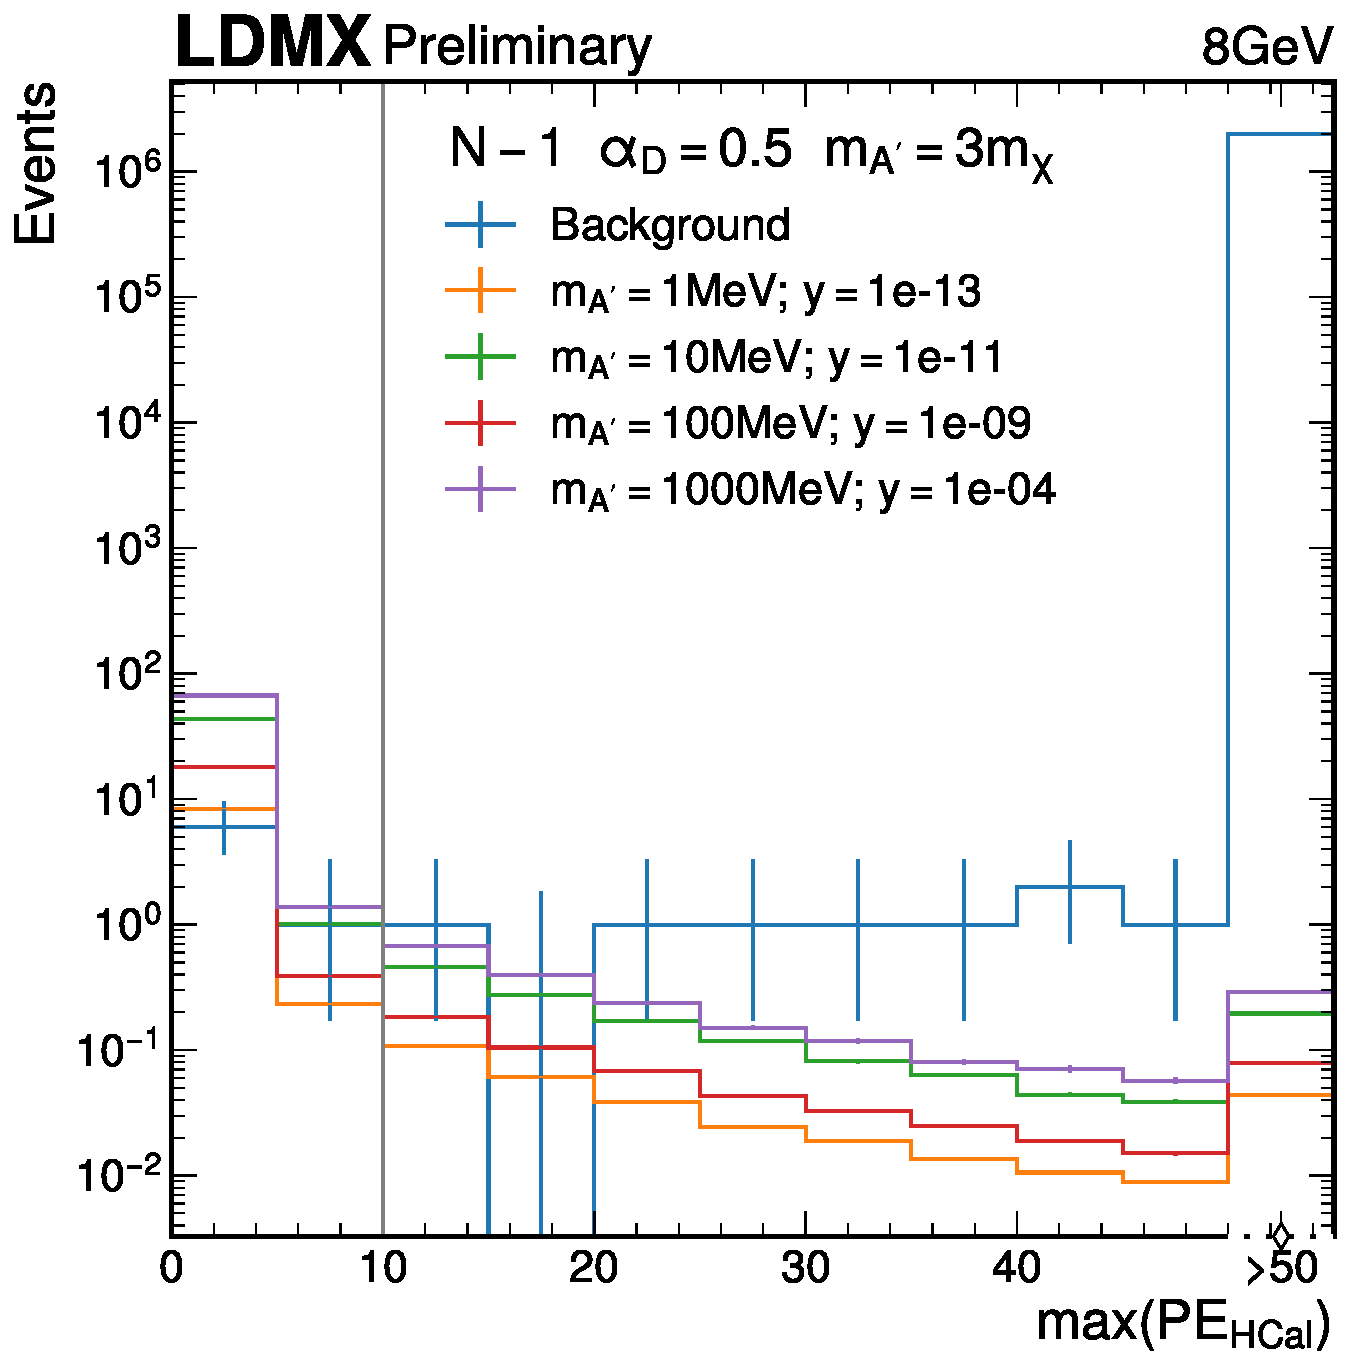
\includegraphics[width=\textwidth]{figures/ldmx/analysis/nm1-hcal-max-pe-8gev-1e13norm.pdf}
    \end{subfigure}
    ~
    \begin{subfigure}{0.48\textwidth}
      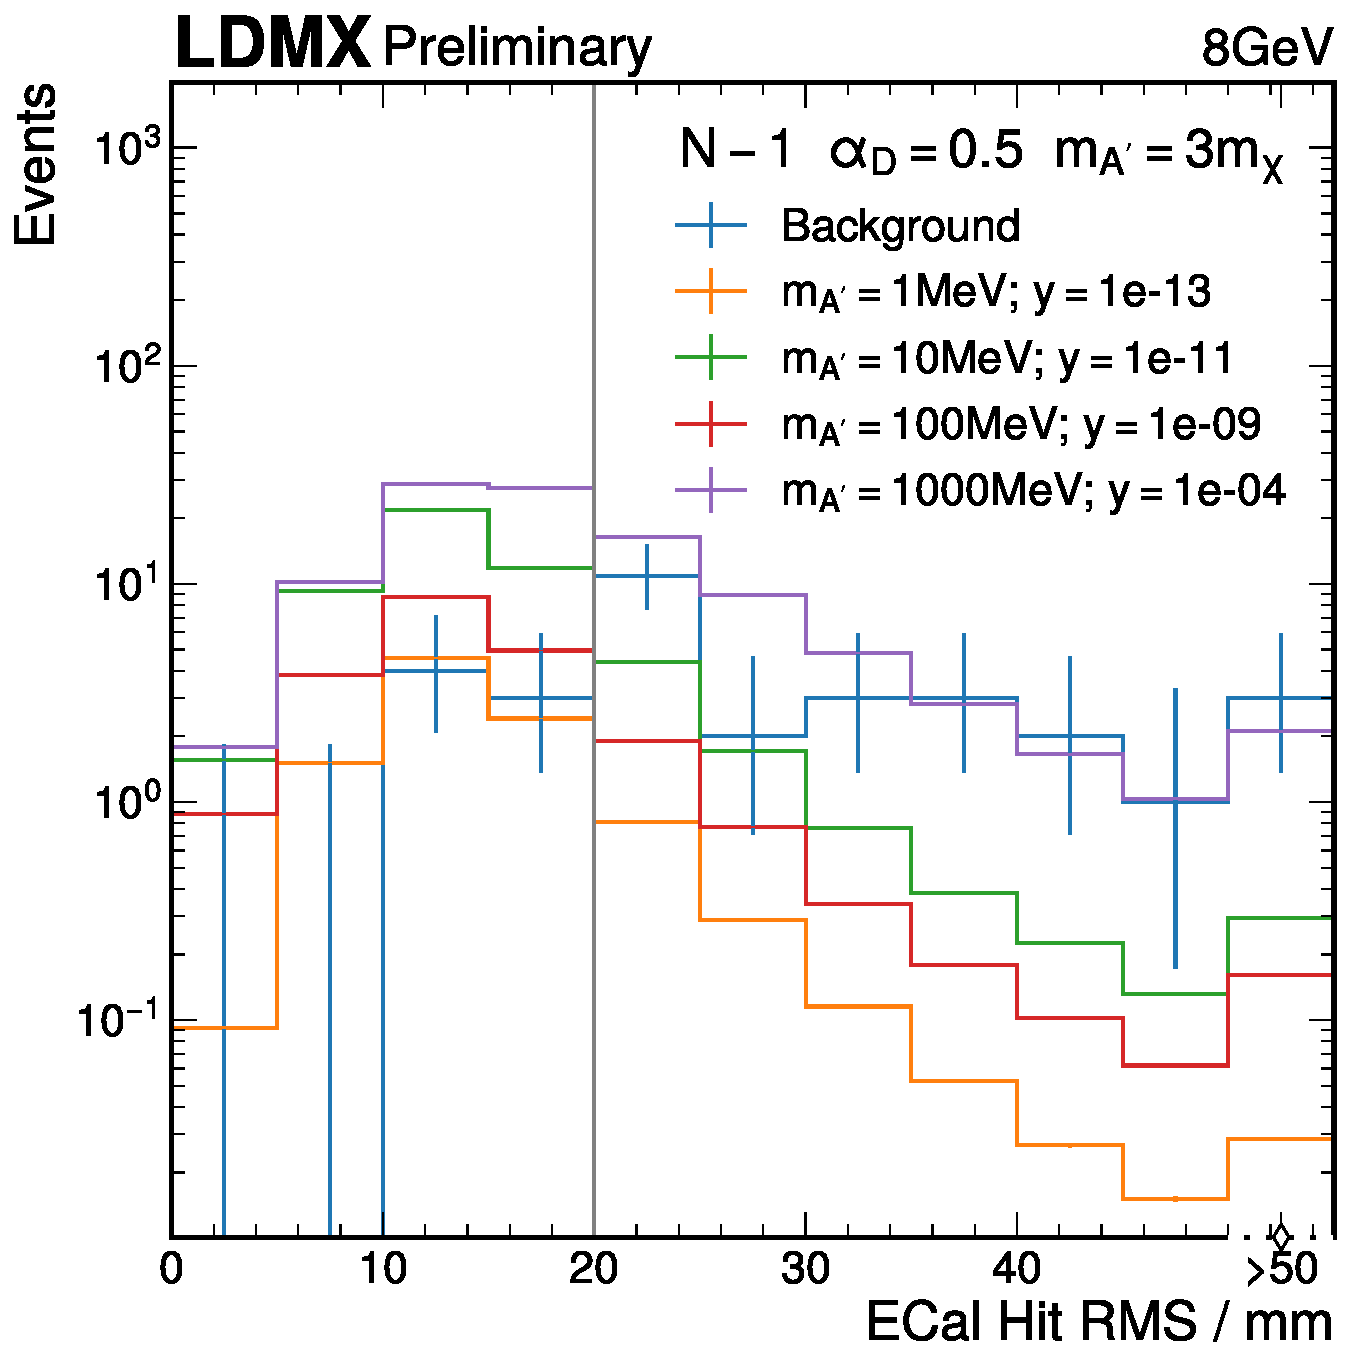
\includegraphics[width=\textwidth]{figures/ldmx/analysis/nm1-ecal-rms-8gev-1e13norm.pdf}
    \end{subfigure}
    \caption{Variables used in signal selection for the \ac{eat} analysis channel.
    In each figure, all other cuts are applied except for the variable in question.
    Some of the bins are empty in which case the upper Poisson limit given the total
    sample size is drawn with error bars.
    The grey line shows the selection cut.
    The background sample is the enriched nuclear and dimuon samples.
    The top (bottom) row shows the \qty{4}{\GeV} (\qty{8}{\GeV}) beam.
    }
    \label{fig:selection-variables}
\end{figure}

\begin{table}[htb]
    \centering
    \begin{tabular}{|r|c||c|c|c|c|}
    \hline
    \multirow{2}{*}{Analysis Stage for \fourgev Beam} & 
      Background & 
      \multicolumn{4}{c|}{Signal Efficiency (\%)} 
      \\ \cline{3-6} 
    & Event Yield & $1$~MeV & $10$~MeV & $100$~MeV & $1$~GeV \\ \hline
    \ecal Trigger ($E_{20} < 1.5$~GeV) &
      \num{4.60e+07} & 58 & 67 & 71 & 83 \\
    \ecal Energy ($E_{\mathrm{\ecal}} < 1.1$~GeV) & 
      \num{1.95e+06} & 35 & 48 & 53 & 72 \\
    $\max(\text{PE}_{\text{\hcal}}) < 10$ &
      \num{1.15e+03} & 34 & 47 & 52 & 69 \\
    ECal Hit RMS $< 20\;\mathrm{mm}$ &
      126 & 28 & 37 & 41 & 33 \\
    \hline
    \hline
    \multirow{2}{*}{Analysis Stage for \eightgev Beam} & 
      Background & 
      \multicolumn{4}{c|}{Signal Efficiency (\%)} 
      \\ \cline{3-6} 
    & Event Yield & $1$~MeV & $10$~MeV & $100$~MeV & $1$~GeV \\ \hline
    \ecal Trigger ($E_{20} < 3.16$~GeV) &
      \num{6.10e+07} & 66 & 74 & 79 & 89 \\
    \ecal Energy ($E_{\text{\ecal}} < 2.76$~GeV) &
      \num{6.88e+06} & 52 & 63 & 69 & 84 \\
    $\max(\text{PE}_{\text{\hcal}}) < 10$ &
      31.8 & 50 & 61 & 67 & 81 \\
    ECal Hit RMS $< 20\;\mathrm{mm}$ &
      7 & 43 & 52 & 56 & 52
    \\ \hline
\end{tabular}

    \caption{
      Cut-flow analysis comparing background and various signal hypotheses for the simple cuts used in this analysis.
      The event yield for the background sample is calculated using the event weights
      and represent the number of events out of $10^{13}$ EoT equivalent.
      The signal efficiency is relative to the full simulation sample.
      The efficiency and event yield values on a given row are for \emph{after} the analysis stage of that row.
      The first table is the cutflow for the \qty{4}{\GeV} beam, and the second table is for the \qty{8}{\GeV} beam.
    }
    \label{tab:cutflow}
\end{table}

\begin{figure}[htb]
    \centering
    \begin{subfigure}{0.48\textwidth}
       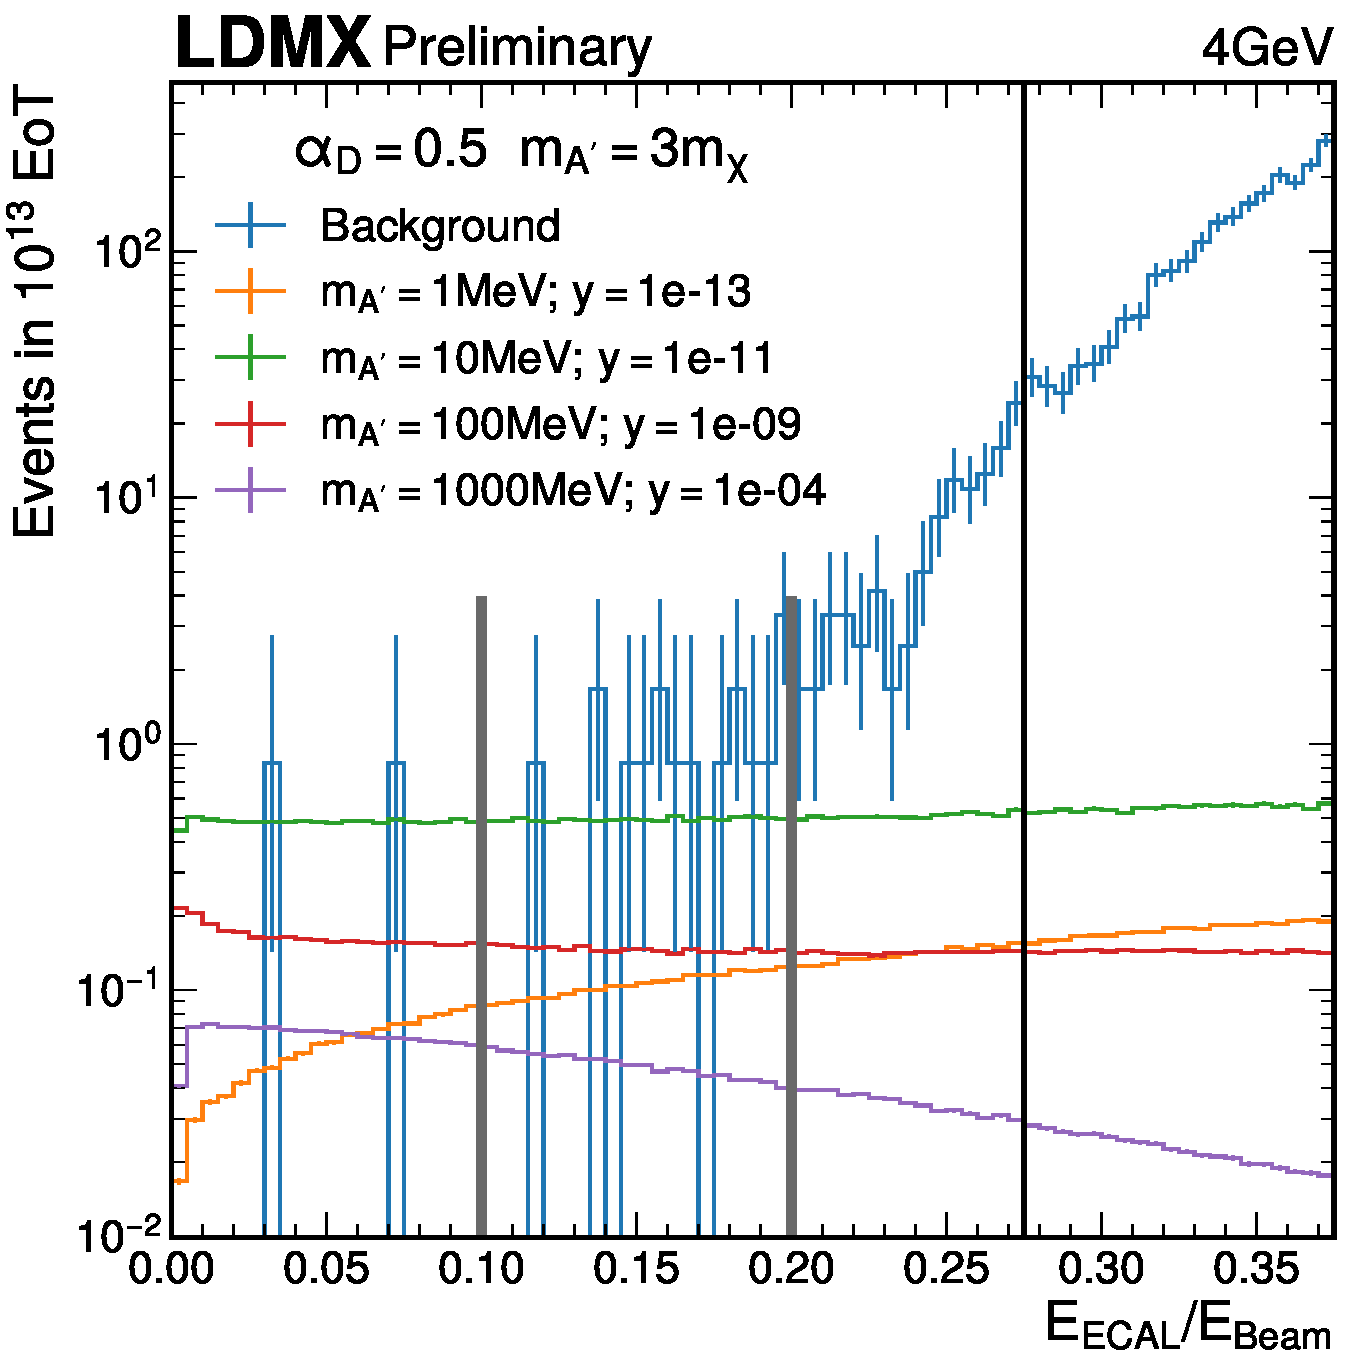
\includegraphics[width=\textwidth]{figures/ldmx/analysis/final-selection-with-ana-bin-edges-4gev.pdf}
    \end{subfigure}
    ~
    \begin{subfigure}{0.48\textwidth}
       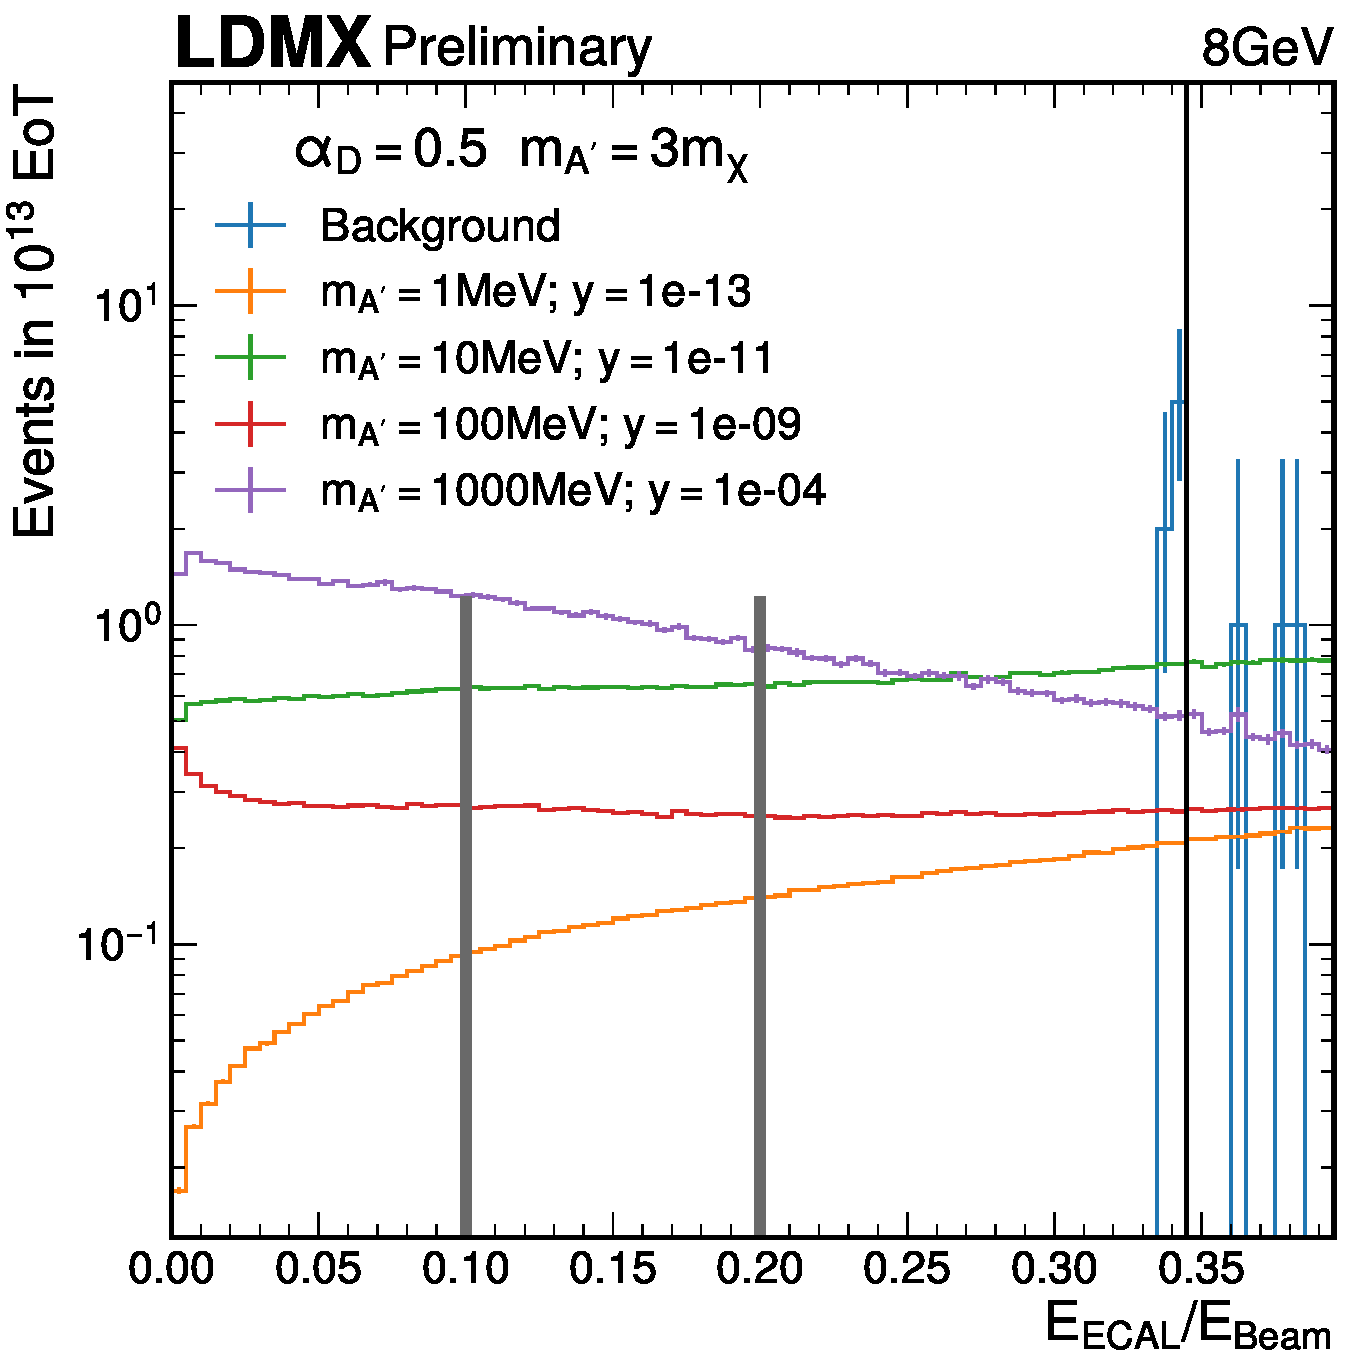
\includegraphics[width=\textwidth]{figures/ldmx/analysis/final-selection-with-ana-bin-edges-8gev.pdf}
    \end{subfigure}
    \centering
    \caption{The total reconstructed energy in all layers of the \ac{ecal} ($E_\text{ECAL}$)
    as a fraction of the beam energy ($E_\text{Beam}$) for all samples that
    pass the selection criteria except the selection on \ac{ecal} energy.
    The \qty{4}{\GeV} beam is shown on the left and the \qty{8}{\GeV} beam is shown on the right.
    The gray lines mark the edges of the analysis bins used to
    estimate the expected exclusion limit and the black line is the upper limit
    on the \ac{ecal} energy which also serves as the upper limit of an analysis bin.
    }
    \label{fig:final-selection}
\end{figure}

\section{Background Prediction}
When performing a search for new processes, a common technique is to develop a well-motivated
prediction for the background processes and then look for excesses above this prediction.
Before we go through rigourously defining what an ``excess'' means and how to quantify
what types of new processes we would exclude if no excess is observed,
we should more precisely define what our background prediction is.

We begin with fitting the cumulative background distribution with a simple exponential function.
\cref{fig:bkgd-fit} shows this cumulative distribution, the resulting fit, and the 95\% confidence
intervals surrounding the fit.
This fit is a helpful prediction tool in two keys ways.
The fit produces a meaningful prediction across the entire range of observable values
which is a helpful way to ``smooth'' out this sample that is limited in size after the selection
criteria already applied.
Moreover, the fit uses the \qty{400}{\MeV}-wide control region between the upper limit on the total
\ac{ecal} energy and the trigger threshold applied during readout to help constrain its parameters.
This constraint reduces the uncertainty on the background prediction while also serving
as an example of what an analysis using real data could do -- this same region could be utilized
in order to help set the scale of the background in a data-driven way.

\begin{figure}[htb]
  \centering
  \begin{subfigure}{0.48\textwidth}
    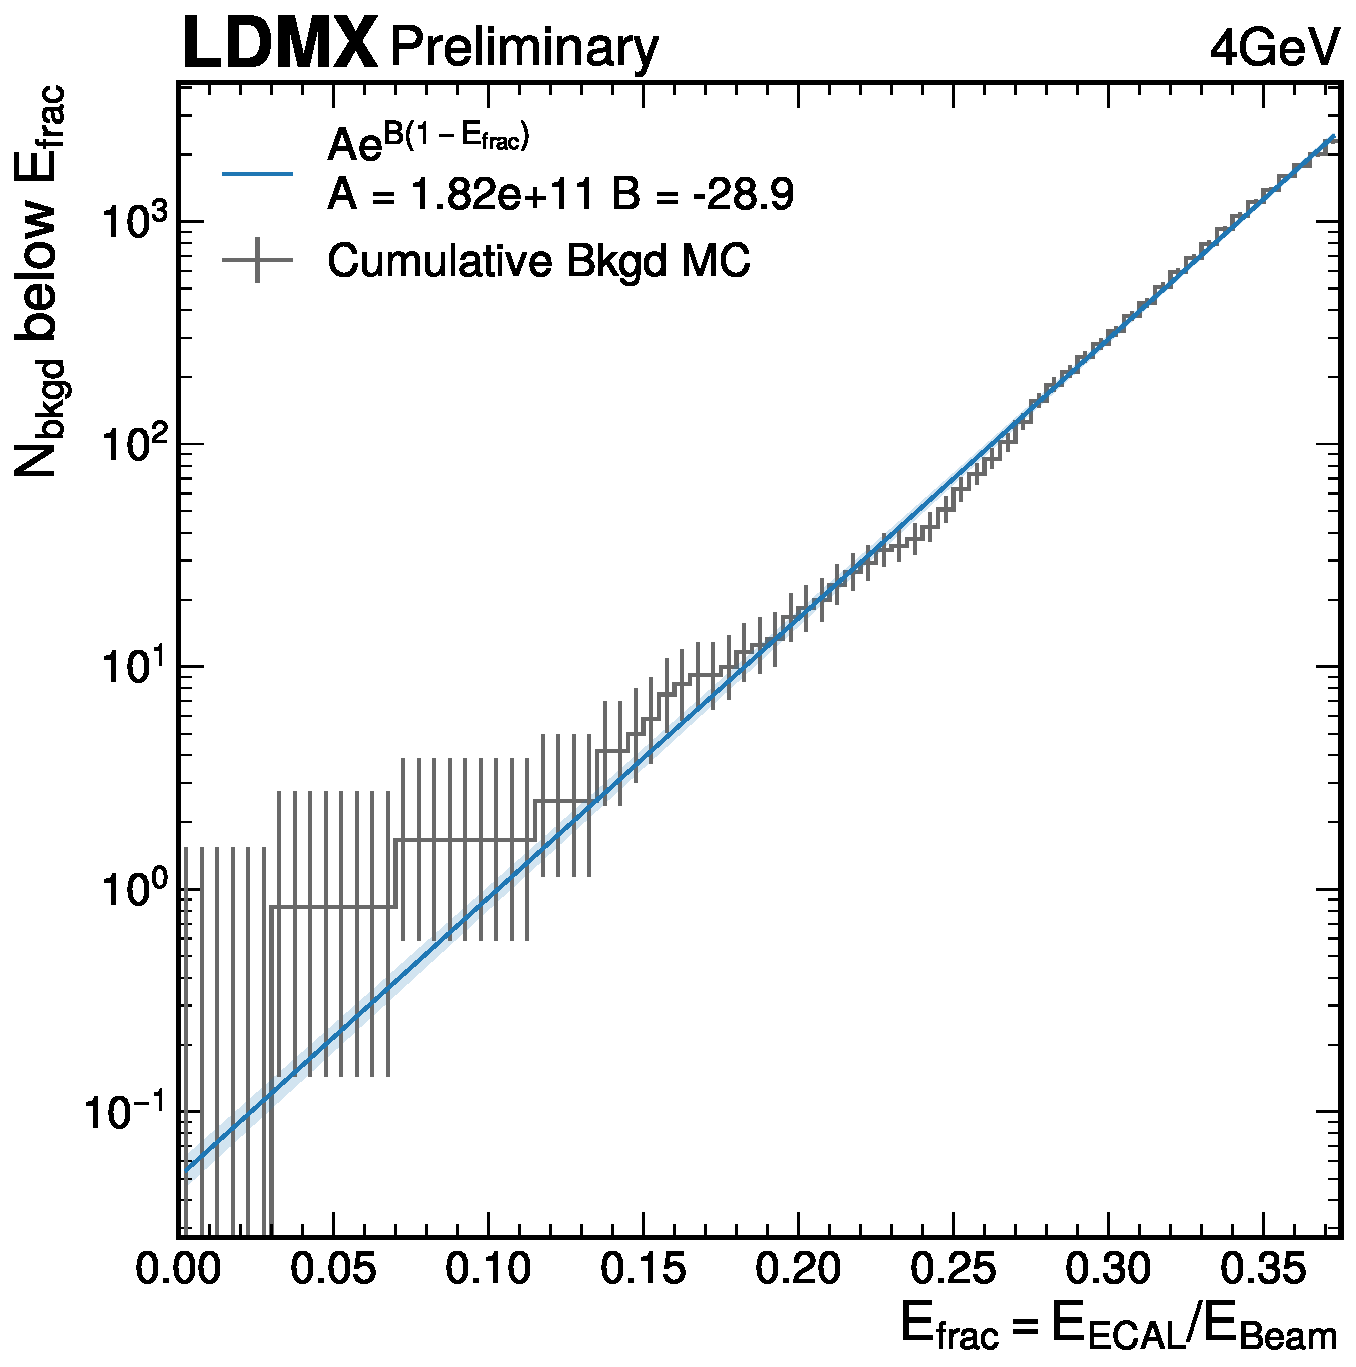
\includegraphics[width=\textwidth]{figures/ldmx/analysis/4gev-cumulative-bkgd-fit.pdf}
  \end{subfigure}
  ~
  \begin{subfigure}{0.48\textwidth}
    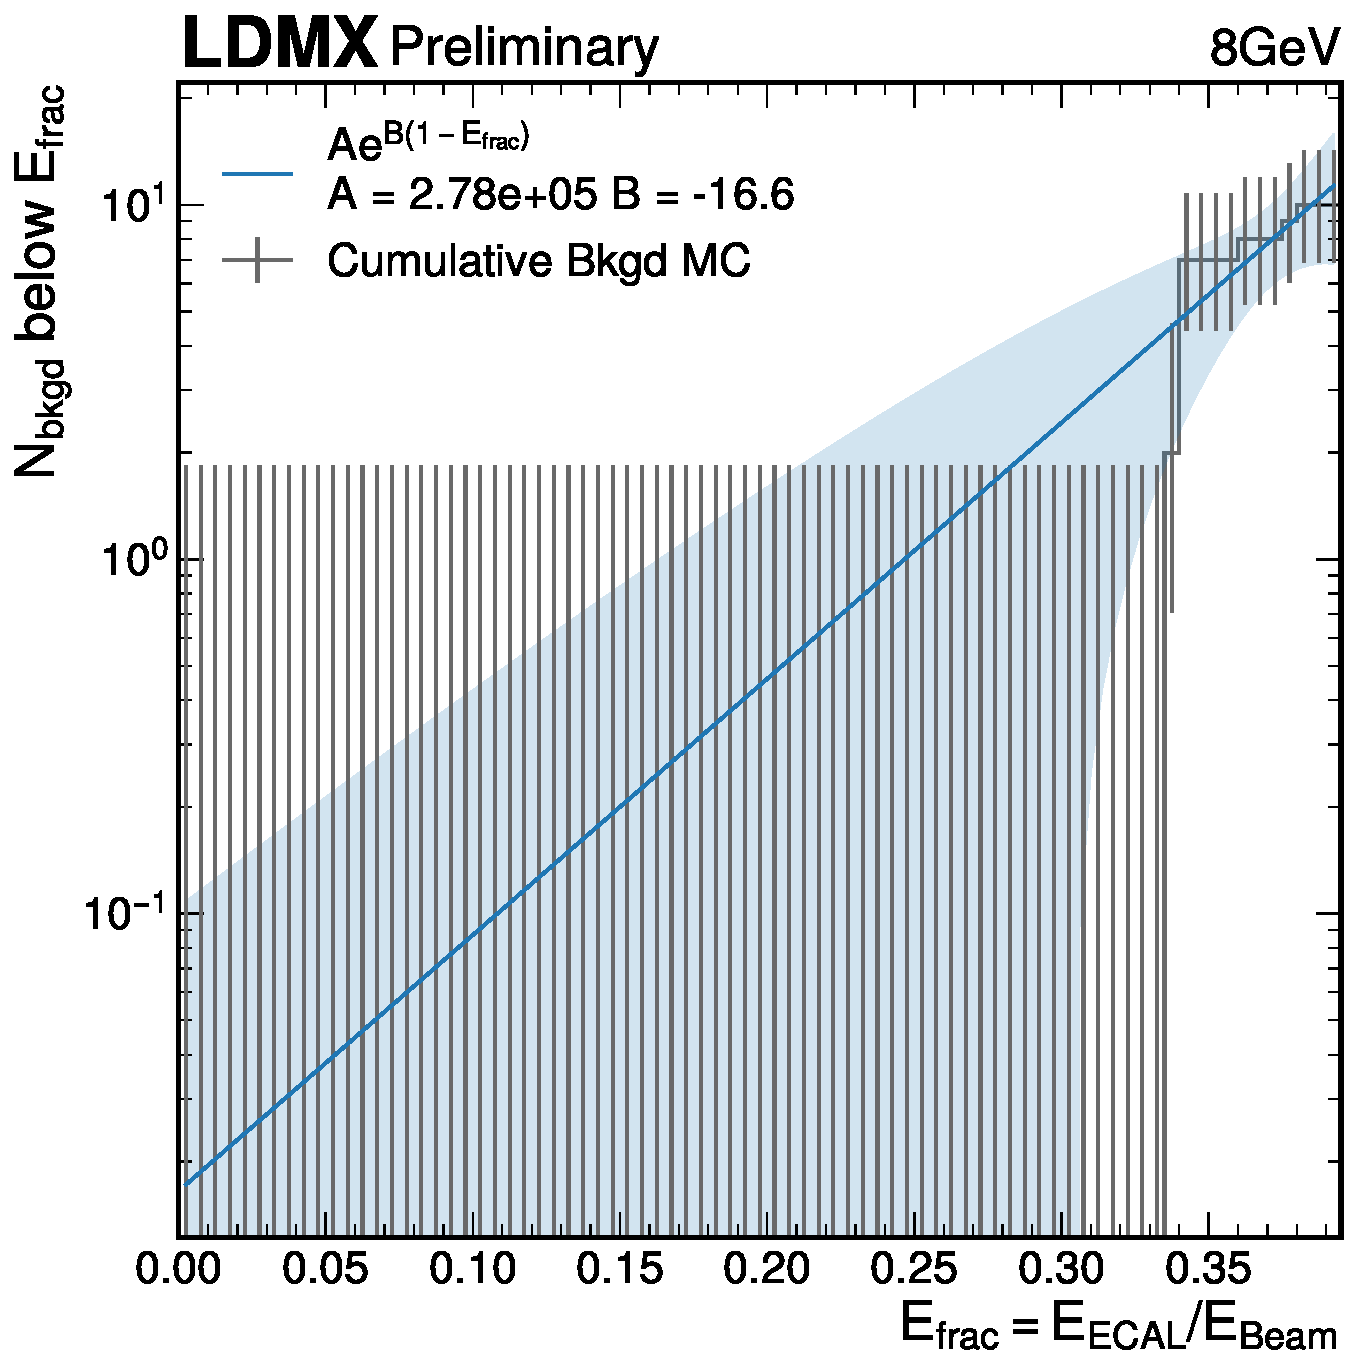
\includegraphics[width=\textwidth]{figures/ldmx/analysis/8gev-cumulative-bkgd-fit.pdf}
  \end{subfigure}
  \caption{%
    Exponential fit of the total simulated background distribution.
    The shaded region is a 95\% confidence band on the fit which is interpreted
    as the uncertainty on the value of the fit.
    Some bins in the simulated distribution are empty in which case the upper Poisson limit
    given the sample size is drawn as an error bar in that bin.
  }
  \label{fig:bkgd-fit}
\end{figure}

The fit is then used to provide a background prediction within each of the three analysis bins,
shown in \cref{fig:bkgd-pred} along with the unconstrained simulation prediction for comparison.

\begin{figure}[htb]
  \centering
  \begin{subfigure}{0.48\textwidth}
    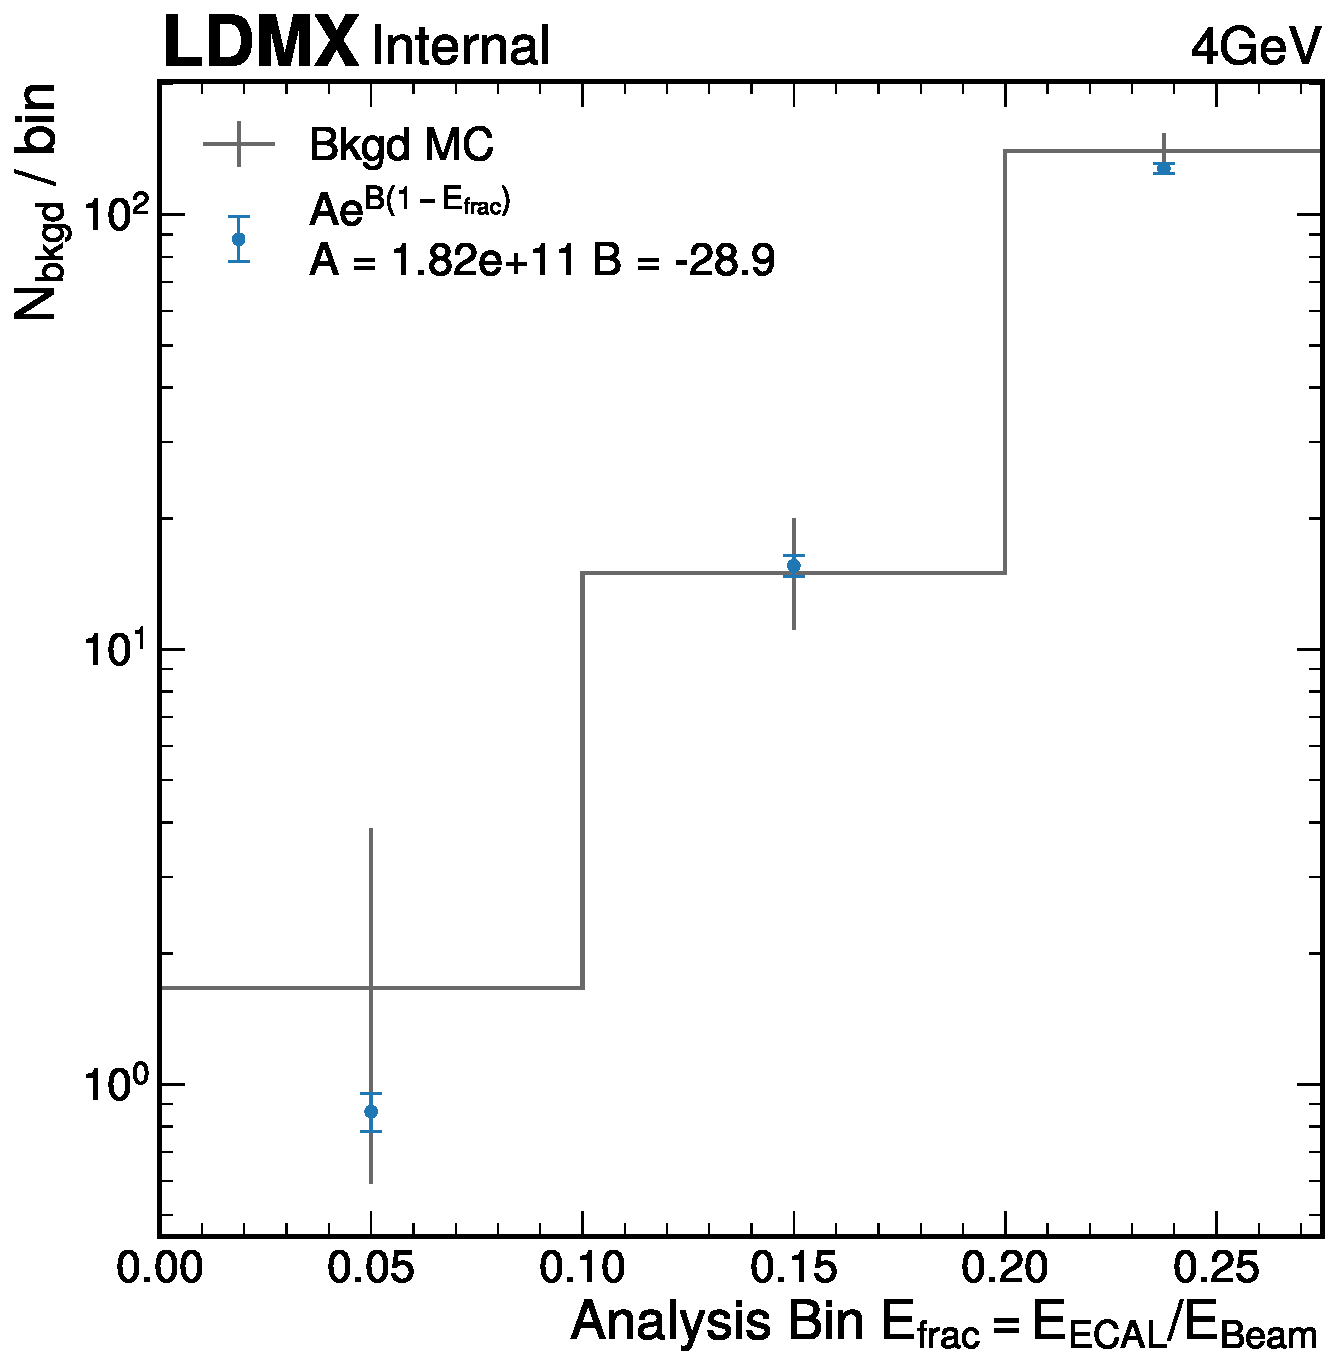
\includegraphics[width=\textwidth]{figures/ldmx/analysis/4gev-integrated-bkgd-fit.pdf}
  \end{subfigure}
  ~
  \begin{subfigure}{0.48\textwidth}
    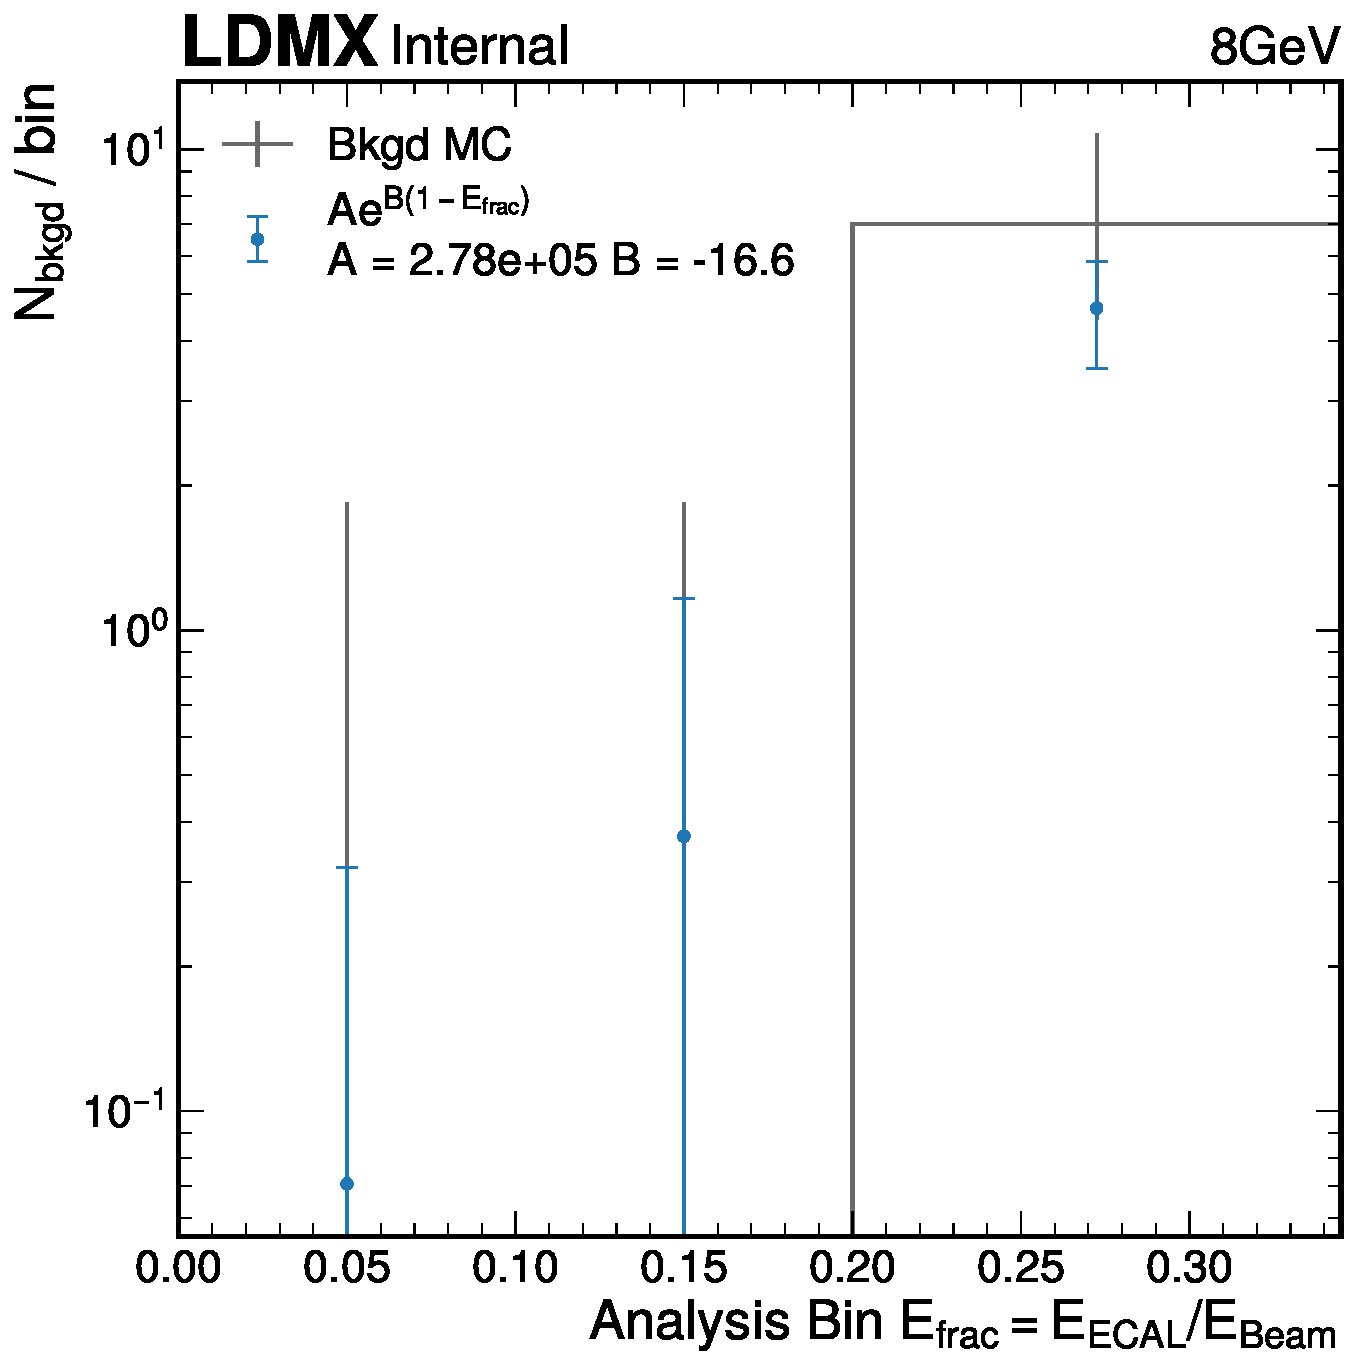
\includegraphics[width=\textwidth]{figures/ldmx/analysis/8gev-integrated-bkgd-fit.pdf}
  \end{subfigure}
  \caption{%
    Background prediction within the three final analysis bins (blue)
    compared to the unconstrained simulation prediction in gray.
    The uncertainty on the background prediction is taken from the 95\% confidence band
    shown on the fit.
    Some bins in the simulation prediction are empty in which case the upper Poisson limit
    given the sample size is drawn as an error bar in that bin.
  }
  \label{fig:bkgd-pred}
\end{figure}

\section{Systematics and Background Uncertainty}
Besides the statistical uncertainty due to the finite size of the simulation sample
(whose estimation is represented by the \qty{95}{\percent} confidence intervals around the fit),
there is additional sources of uncertainty that originate from the experimental design
(so-called ``systematic'' uncertainty).
Most prominently in this early-running analysis, we expect mis-calibration of the \ac{ecal}
to be a potentially major source of systematic uncertainty especially since the calibration
of the \ac{ecal} used when applying the trigger selection will probably differ from the
calibration used later on during the final analysis.\footnote{
  This difference is expected since we can improve the calibration of the detector as we
  collect more data; however, acknowledging this difference helps us put requirements on
  the accuracy of the intial calibration used at the trigger level in order for this
  analysis to function as expected.
}
Estimating this systematic uncertainty is rather direct; we simply vary the calibration
used at the reconstruction and analysis stage within our data processing and see how that
changes the results.\footnote{
  The estimate for both the \ac{ecal} and \ac{hcal} systematics is done with the
  \qty{4}{\GeV} beam sample since that estimate is expected to be more conservative
  because the \qty{4}{\GeV} beam sample allows more background yield past its selections
  compared to the \qty{8}{\GeV} beam sample.
}

We generated ten different calibrations, smearing the calibration constants by \qty{10}{\percent}
in an uncorrelated fashion and by an additional, correlated \qty{2}{\percent} (\qty{5}{\percent})
within the central (outer) modules of the \ac{ecal}.
These smearing factors are a conservative estimate of the accuracy of the initial calibrations
used by the trigger to make data collection decisions.
These ten different calibrations were then used to re-reconstruct the simulated events
ten different times yielding \cref{fig:4gev-smeared-unsmeared-comp}
and \cref{fig:4gev-smeared-unsmeared-ecal-hit-rms}.
\cref{fig:4gev-smeared-unsmeared-comp:fail-trigger} reassures us that our signal region
(below \qty{1.1}{\GeV}) is not polluted with events that would have failed the trigger
selection even after these rather large calibration changes relative to the trigger calibrations
(i.e. we would not have overestimated our signal efficiency).
In addition, we can estimate the resulting systematic variation on the background
event yield within the three final analysis bins to be \qty{5}{\percent} using
\cref{fig:4gev-smeared-unsmeared-comp:pass-trigger}.
The final selection on the \ac{ecal} Hit RMS is only affected negligibly as shown in
\cref{fig:4gev-smeared-unsmeared-ecal-hit-rms} where the distribution only chagnes by
$\lesssim\qty{5}{\percent}$ within the range of potential cuts.

\begin{figure}
  \centering
  \begin{subfigure}[t]{0.48\textwidth}
    \centering
    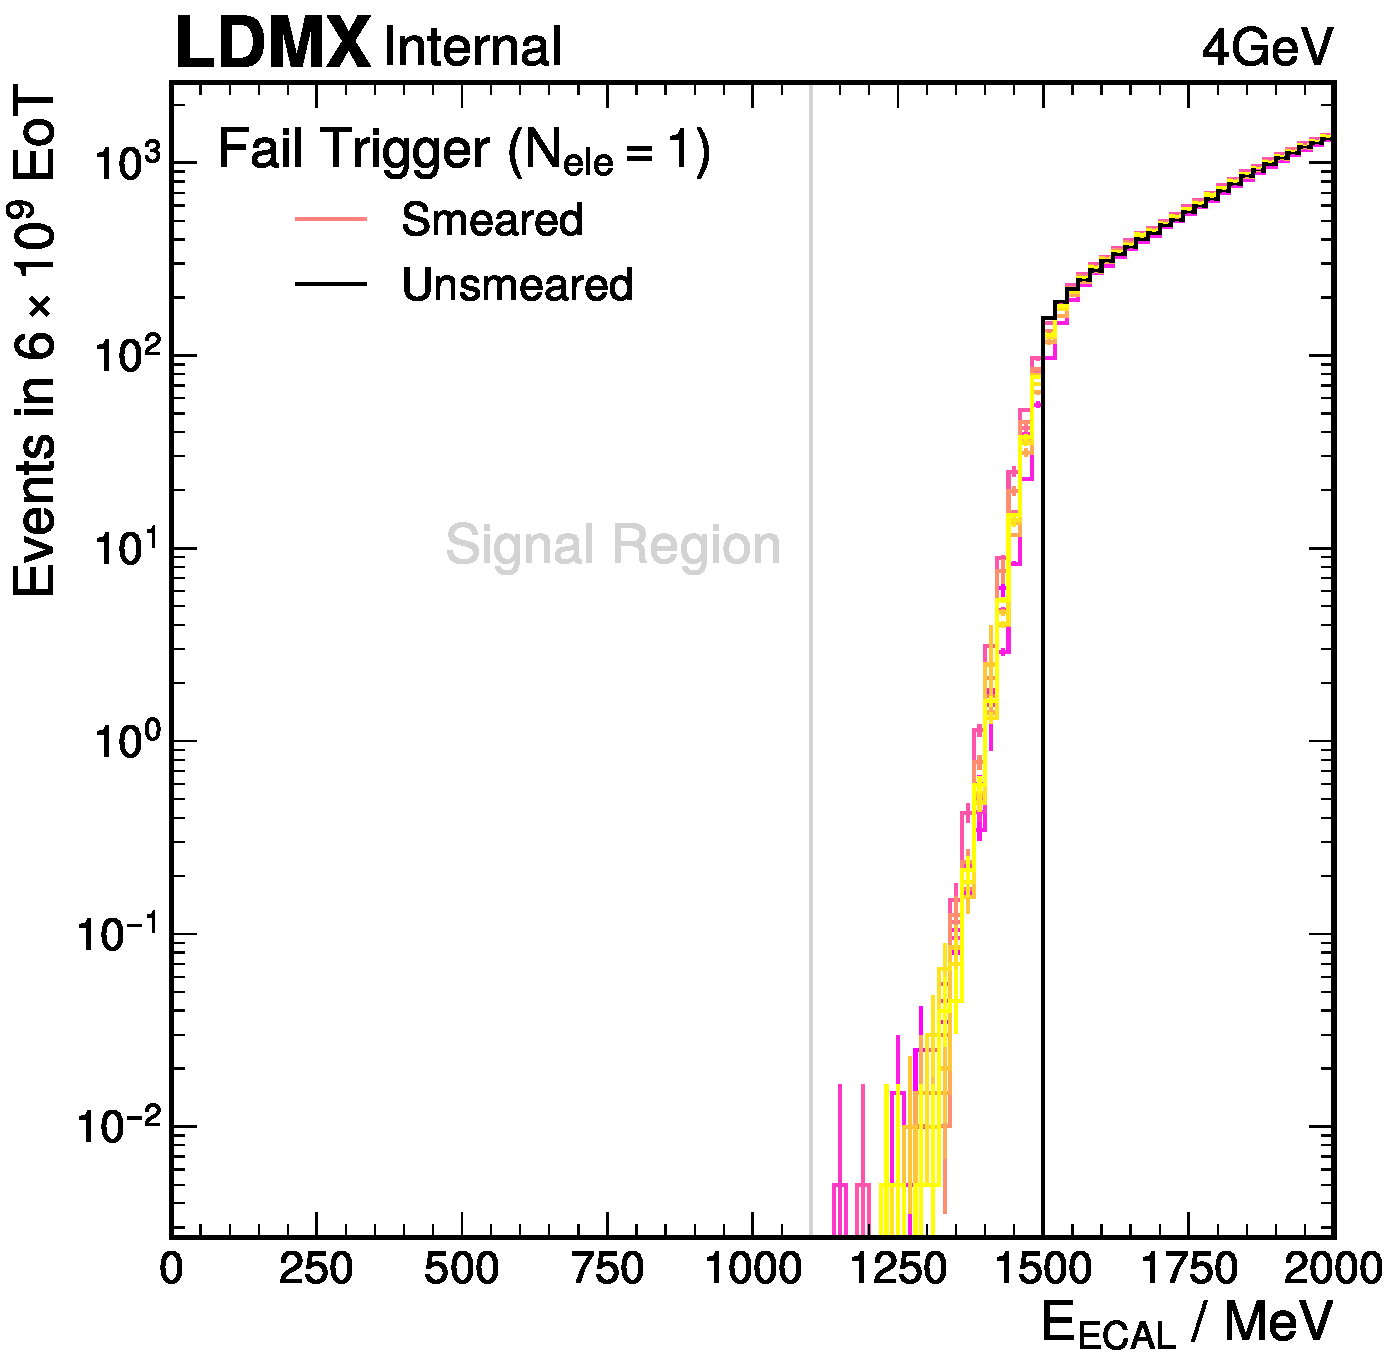
\includegraphics[width=\textwidth]{figures/ldmx/analysis/systematics/4gev-fail-trigger-uncorrcell.pdf}
    \caption{Events failing the original trigger.}
    \label{fig:4gev-smeared-unsmeared-comp:fail-trigger}
  \end{subfigure}%
  ~
  \begin{subfigure}[t]{0.48\textwidth}
    \centering
    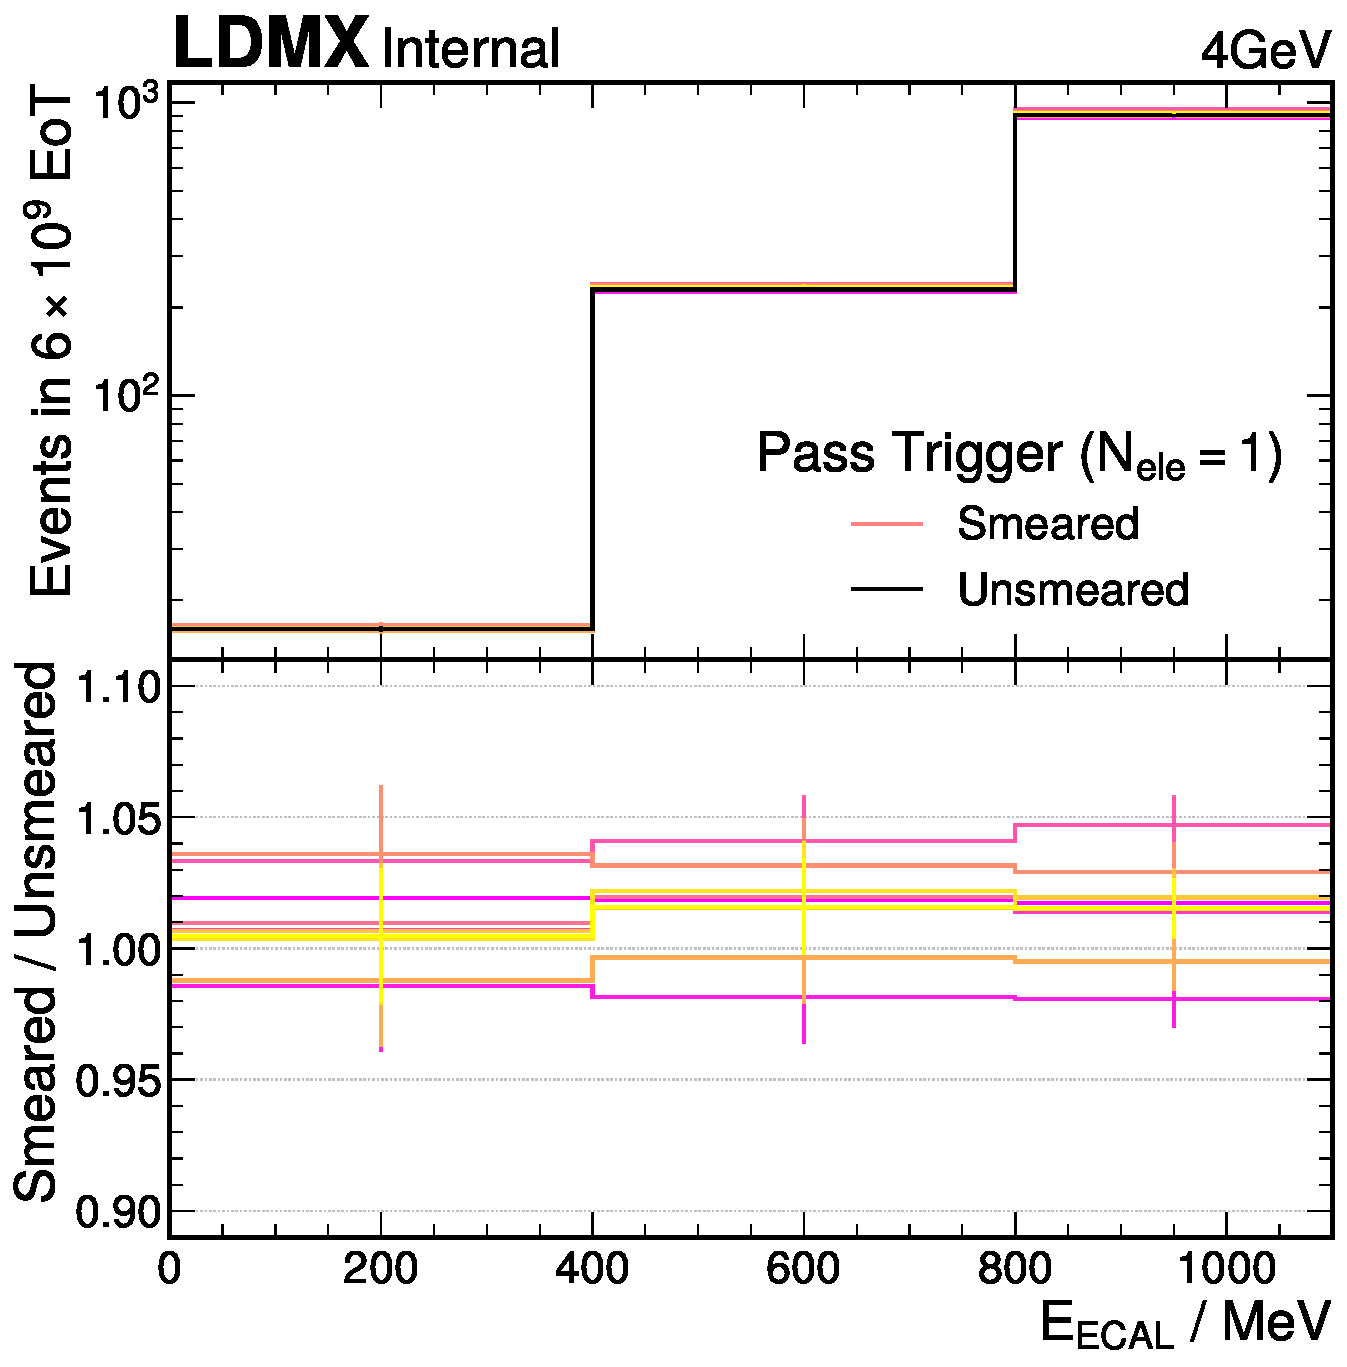
\includegraphics[width=\textwidth]{figures/ldmx/analysis/systematics/4gev-pass-trigger-ana-bins-uncorrcell.pdf}
    \caption{Events passing the original trigger and falling within one of the three
    final analysis bins over $E_\text{ECAL}$.}
    \label{fig:4gev-smeared-unsmeared-comp:pass-trigger}
  \end{subfigure}
  \caption{The total reconstructed energy in the \ac{ecal} $E_\text{ECAL}$ comparing 
  ten different smeared calibrations (colors) to the original unsmeared calibrations
  (black).}
  \label{fig:4gev-smeared-unsmeared-comp}
\end{figure}

\begin{figure}
  \centering
  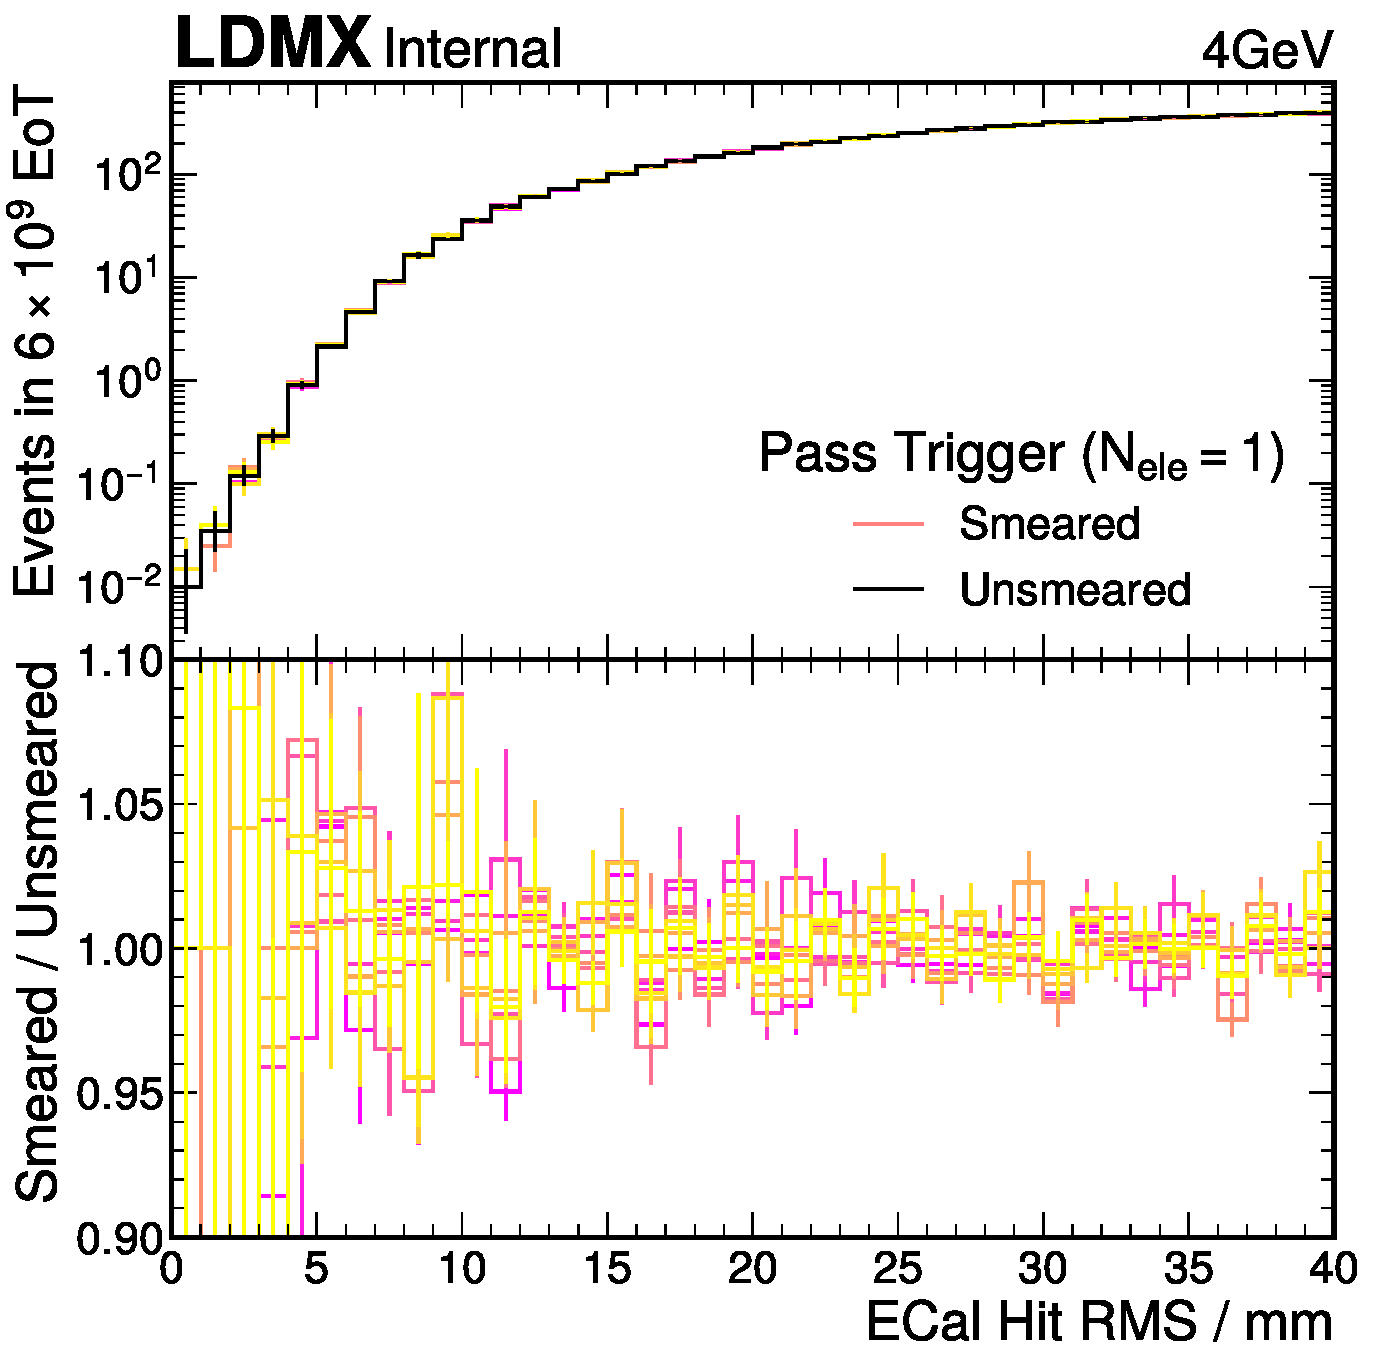
\includegraphics[width=0.5\textwidth]{figures/ldmx/analysis/systematics/4gev-pass-trigger-uncorrcell-ecal-hit-rms.pdf}
  \caption{Effect of smeared \ac{ecal} calibrations on the \ac{ecal} hit RMS for events
  that pass the original trigger.
  Outside of statistical fluctuations in the lowest-populated bins, the smearing has
  a less than 5\% effect throughout the range of potential cuts.}
  \label{fig:4gev-smeared-unsmeared-ecal-hit-rms}
\end{figure}

Estimating the systematic uncertainty due to the \ac{hcal} variable is not as
straight forward since we are unsure on how best to directly alter the conditions
with which the \ac{hcal} is reconstructed.
We can still estimate the systematic uncertainty due to this cut variable
by testing a wide range of cut variables, deducing which ones
are ``acceptable'' and then extracting how the background yield varies between these
different cut choices.
(What we want to be emulating is the underlying distribution shifting relative
to our analysis cut, but we are mimicing this by shifting the cut relative to the
distribution.)

\begin{figure}
  \centering
  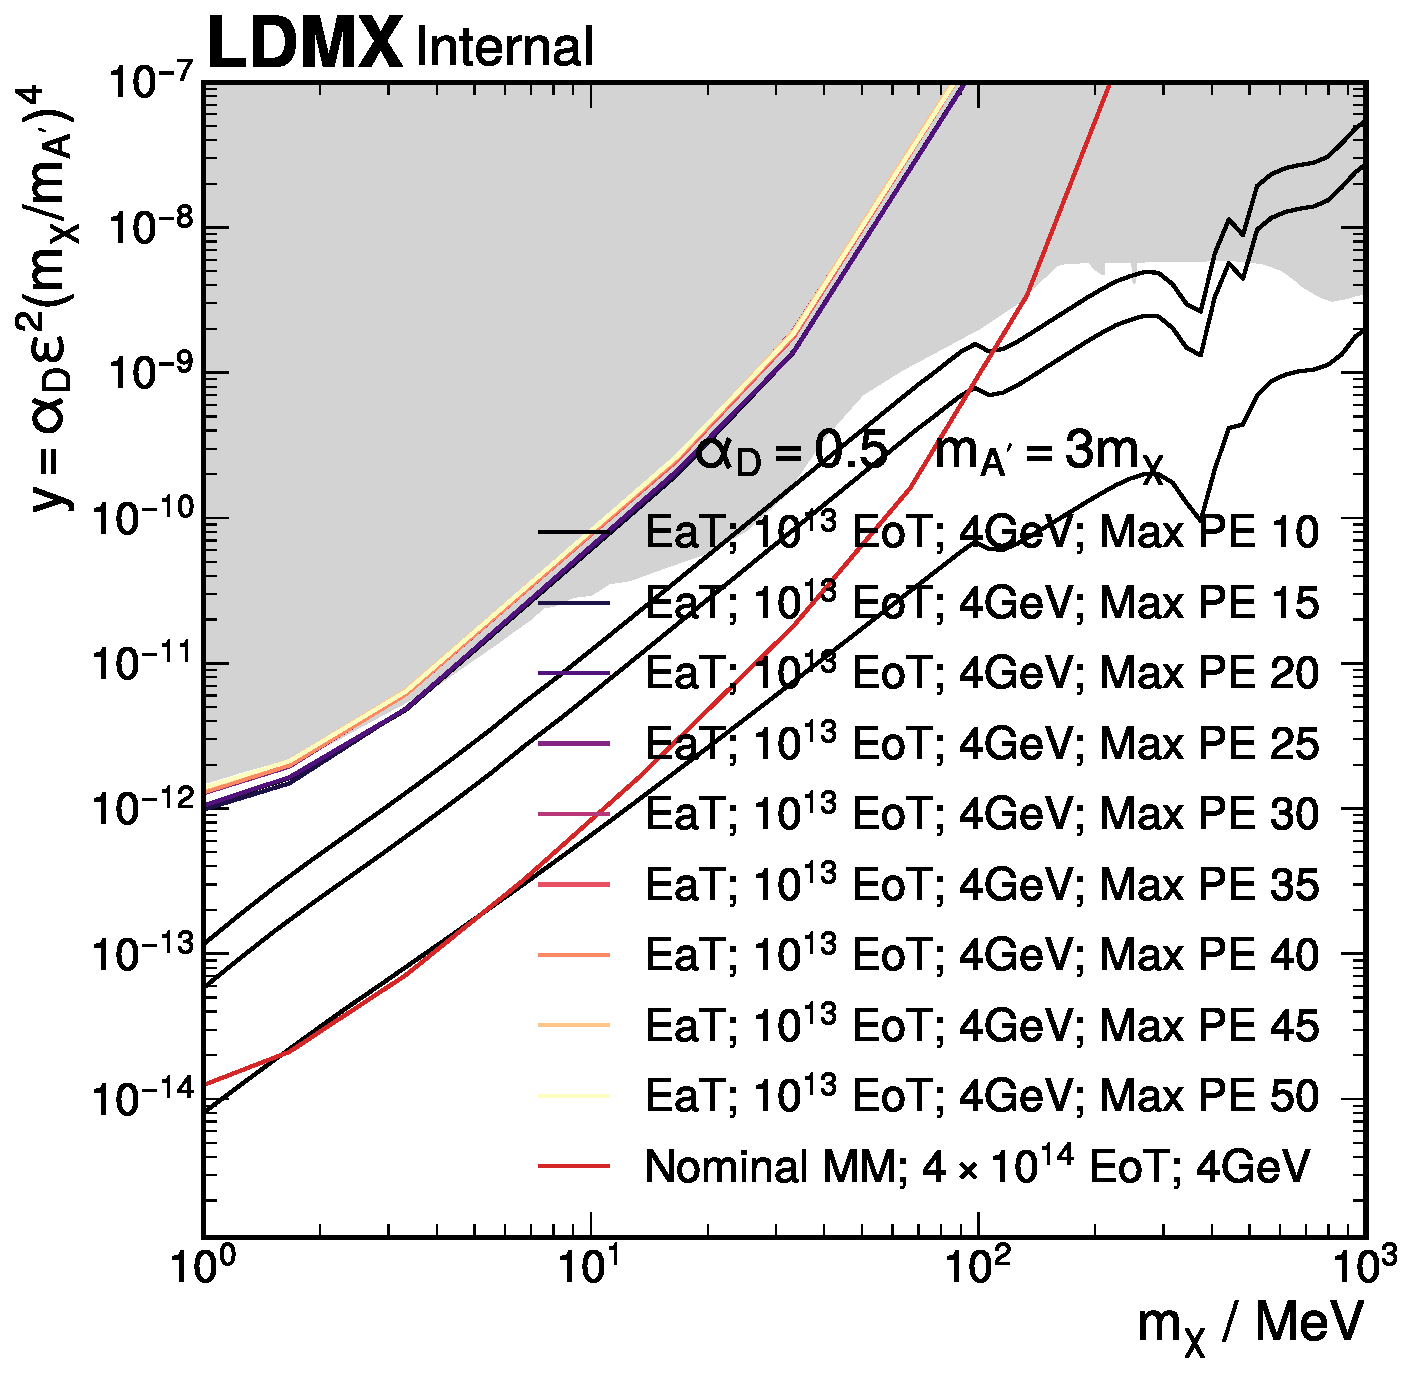
\includegraphics[width=0.5\textwidth]{figures/ldmx/analysis/systematics/max-pe-scan-4gev.pdf}
  \caption{Various reach lines for the 4GeV beam case as we vary the cut on
  maximum \ac{hcal} PE. We observe minimal movement in the final reach as a function
  of this cut; nevertheless, the biggest change occurs around a threshold of 30.}
  \label{fig:4gev-max-pe-scan}
\end{figure}

Figure \ref{fig:4gev-max-pe-scan} shows how the final reach (see \cref{sec:ldmx:analysis:reach})
changes depending on this cut.
While not much movement is observed, we can see separation ocurring when the threshold
goves above $\sim 30$.
With this in mind, we estimate our ``tolerance'' to a systematic error on the maximum
\ac{hcal} PE to be $1 - B_{< 10}/B_{< 20}$ where $B_{< M}$ is the background yield
with the maximum \ac{hcal} PE threshold $M$.
This yields an analysis-bin-dependent systematic uncertainty of $0.0$, $0.6$, and $0.7$
for the low, medium, and high $E_\text{frac}$ analysis bins respectively.

\section{Reach}
\label{sec:ldmx:analysis:reach}
We can quantitatively define an excess above a background prediction using statistical techniques
like a one-sided Poisson-distributed p-value test; however, in this context it is often more helpful
to characterize the signal models that would be excluded if the data was collected and it aligned
with the background prediction.
These ``exclusion estimates'' (colloquially referred to as ``reach'') rely on statistical tools
that are common within \ac{hep} and implemented within \textsc{Combine}\cite{cms-combine}.
\cref{fig:4gev-max-pe-scan} has already shown an example reach that varies depending on the value
of the cut we choose to use during the selection; however, the final reach including the statistical
and systematic uncertainties discussed above is shown in \cref{fig:reach}.
The \ac{ldmx} \ac{eat} analysis channel is able to search through previously-unexplored phase space
utilizing simple, physically-motivated cuts and $\sim \qty{2.5}{\percent}$ of the planned \ac{eot}
for the first phase of \ac{ldmx}

\begin{figure}
  \centering
  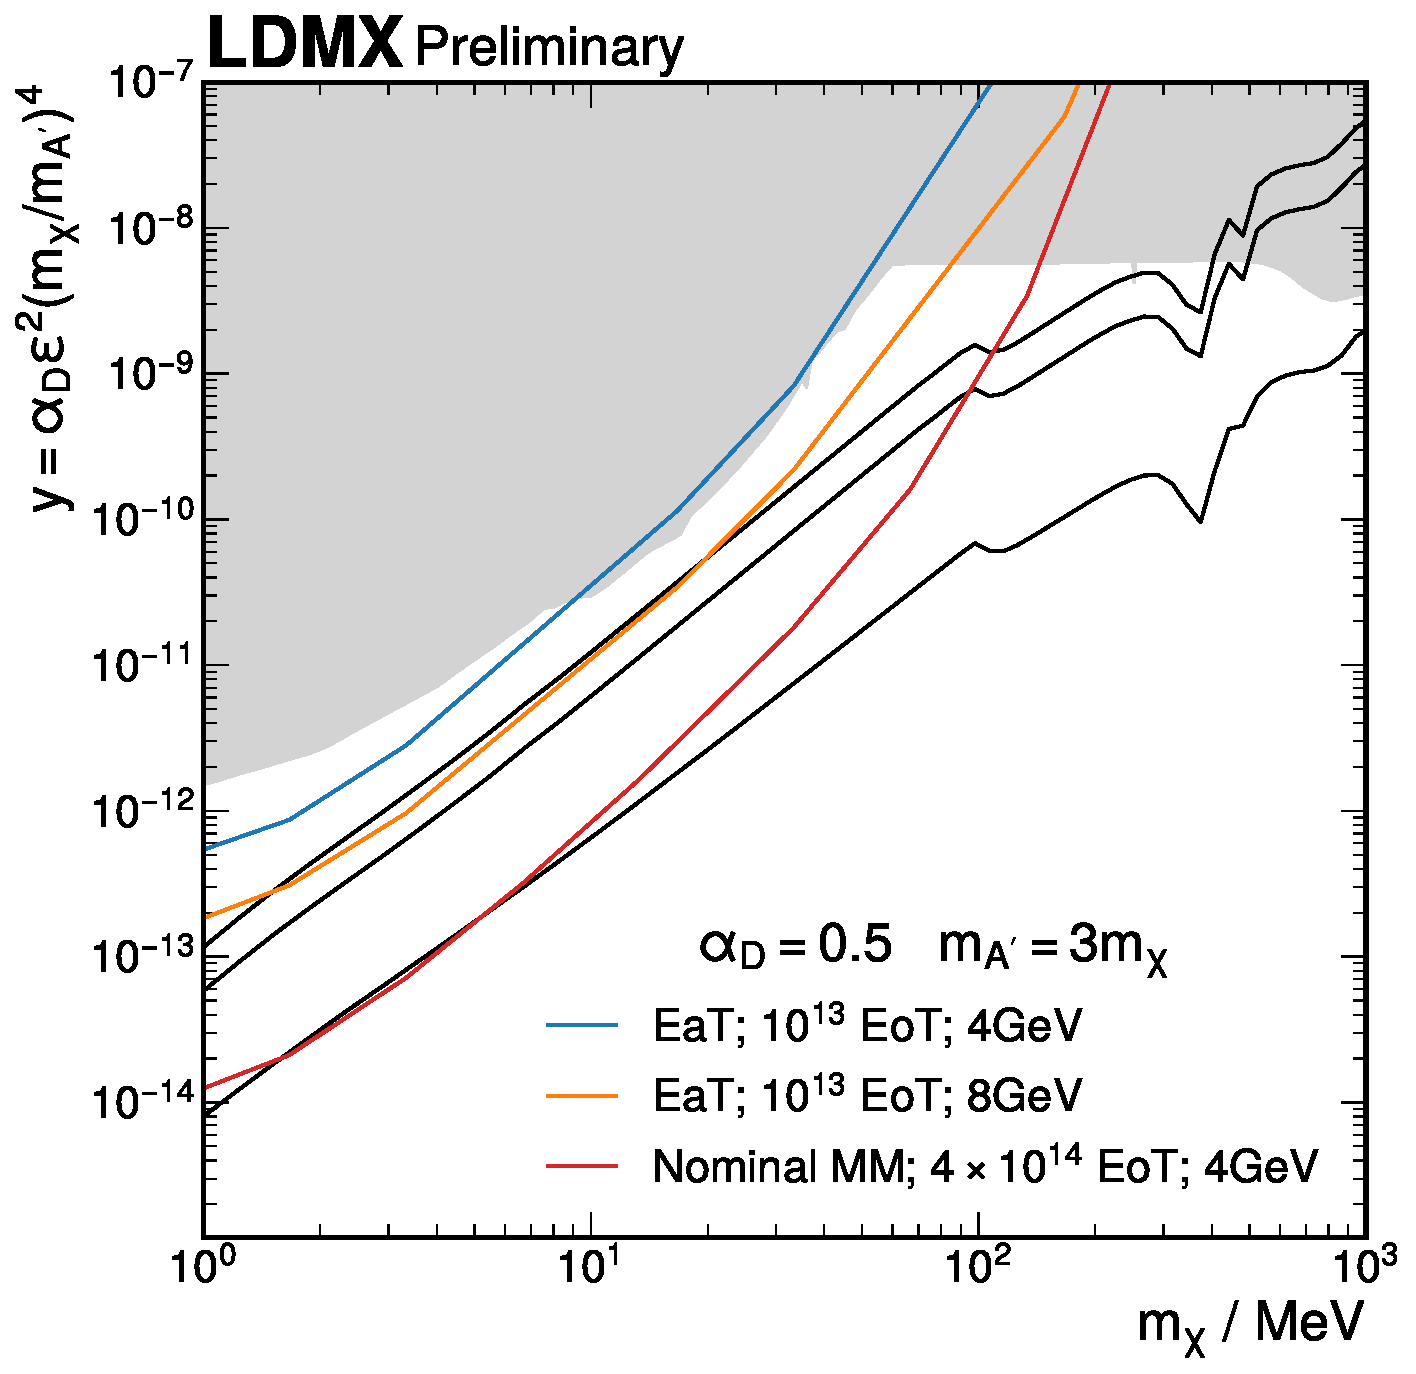
\includegraphics[width=0.5\textwidth]{figures/ldmx/analysis/reach.pdf}
  \caption{%
    The sensitivity of the \ac{eat} analysis channel compared to
    other experiments (gray), various theories (black), and \ac{ldmx} projections (colors).
    The blue (orange) line corresponds to the \qty{4}{\GeV} (\qty{8}{\GeV}) beam studied in this work.
    The red line is the nominal LDMX analysis sensitivity.
  }
  \label{fig:reach}
\end{figure}
